\section{No uncertainty}
\subsection{Single run analysis}
In order to observe the algorithm's behavior a detailed analysis of a single
run is presented in this section. The problem being analyzed is the
two-criteria binary knapsack problem (see [inref]). The problem is simple and
the number of criteria small in order to focus on the algorithm. Moreover, no
uncertainty in the form of interval coefficients is considered.

Although this section is illustrated only by an example of a single run on the
single problem the conclusions drawn here apply globally. Compare with
further sections of the chapter.

The algorithm runs with default parameters (see [inref]). Exterior loop was
repeated ten times. This means that ten times results (in the form of
solutions) were presented to the (mocked) decision maker. The Results were
recorded.

The same problem was solved in an exact way by a mathematical programming
solver (glpk~[ref]). One used the supposed utility function as an optimisation
goal for the solver. In this way the optimal solutions were obtained (for the
considered instance the best supposed utility function value is
$4154.441453$).

The results of the run from the exterior loop perspective are given in
figure~\ref{c2_utilouter}. All of the results generated during the interior
loop run were recorded. On the chart one can see the best and the worst
solutions in a given run (the rest lies between them). Moreover the best of
the solutions shown to the DM is presented (labeled as ``last''). This is
because for evolutionary algorithm it is possible to find and then forget
``good'' solutions (note that the optimization --- the internal loop --- is
not aware of the supposed utility function, it only tries to approximate it
using induced decision rules). However most of the times the ``last'' solution
equals the ``best'' solution which is good.

One can see that in every iteration there is an improvement, however the
improvements are getting smaller and smaller. This is because the better the
solutions' population, the harder it is to optimize it further.

Now the analysis of the interior loop is given. The first, third and seventh
interior loop will be presented. Other runs are similar, so they were omitted
in the paper. The results are presented in figures \ref{c2_utilgen_01},
\ref{c2_utilgen_03} and \ref{c2_utilgen_07}. The iterations of the interior
loop are also called \textit{generations} because of their evolutionary
nature.

On the charts one can see supposed utility function dependent on a
generation. Also value of the primary score is included for reference. To
recapitulate --- the better the solution fits to induced decision rules, the
higher the primary score; in case of a draw (i.e. the primary score for two
individuals is the same) secondary score is considered.

The improvement happens on the generation basis --- in every iteration the
supposed utility function is getting better. However, as one can see
improvement of the primary score happens mainly at the beginning. The runs
like the one in \ref{c2_utilgen_07}, where the breakthrough is at the end of
the run are in fact rare. Nevertheless the algorithm should not be shut down
after reaching maximum primary score. Although preference information
extracted before the run is now exploited, an improvement can still
occur. More importantly the diversification effort is ongoing now --- when the
primary score (rule based) of all the population is identical, then the
secondary score (distance based --- the less the solution is crowded the
higher the score) starts to play major role in the process, pushing
individuals in the population to new areas in solution space. This can result
in major a breakthrough --- the population may acquire traits wanted by the
DM.

Rules driving the interior loops are presented below

\begin{description}
  \item{\textbf{Iteration 1}} \\
    value$_1 \ge 859.86 \Rightarrow \text{class} \ge \texttt{GOOD}$ \\
    value$_2 \ge 814.71 \Rightarrow \text{class} \ge \texttt{GOOD}$
  \item{\textbf{Iteration 3}} \\
    value$_1 \ge 1023.62 \Rightarrow \text{class} \ge \texttt{GOOD}$ \\
    value$_2 \ge 1011.61 \Rightarrow \text{class} \ge \texttt{GOOD}$
  \item{\textbf{Iteration 7}} \\
    value$_1 \ge 1211.14 \Rightarrow \text{class} \ge \texttt{GOOD}$ \\
    value$_2 \ge 1210.63 \Rightarrow \text{class} \ge \texttt{GOOD}$
\end{description}

Note that there are only two classes --- \texttt{GOOD} and \texttt{NOT GOOD}
so essentially $\text{class} \ge \texttt{GOOD}$ means $\text{class} =
\texttt{GOOD}$.

In order to verify how the rules influence the algorithm's behavior, charts
were prepared (fig.~\ref{c2_valweight_01}, \ref{c2_valweight_03} and
\ref{c2_valweight_07}). For two-criteria problem it is possible to present the
search space on two-dimensional chart.

The iterations $1$ and $3$ show a typical run. Before the 10th generation the
whole population moves to an area covered by the rules. In the further
generations diversification occurs. The 7th iteration is a bit different
though. The evolution not ``discovered'' a way to match the second rule before
the 20th generation. Soon after individuals covering both solutions were
included the whole population drifted to the region marked by both rules.

It can be also insightful to see the mocked DM's choices and compare them with
the inferred rules. They are presented in charts (fig.~\ref{c2_dmchoices_01},
\ref{c2_dmchoices_03}, \ref{c2_dmchoices_07}). It is the case that the choices
directly affected the rules. One can also see another interesting trait of the
problem. The further (in objective space) the selected individuals are, the
harder it is to achieve maximal possible primary score.

Finally, charts presenting how the supposed utility and primary score changed
in the population along with succeeding generations (fig.~\ref{c2_utilind_01},
\ref{c2_utilind_03} and \ref{c2_utilind_07}) are given. They support the
conclusions stated above.

Analysis of single run is a good tool for understanding the internals of the
method and inspecting the method's behavior. One can draw conclusions and spot
potential problems and possible improvements. However, more experiments have to
be conducted and their results should be aggregated using statistical methods
in order to check how useful the method is and what the influence of the
algorithm parameters is. This is done in the further sections.

%% Charts
\begin{figure}[tb]
  \centering 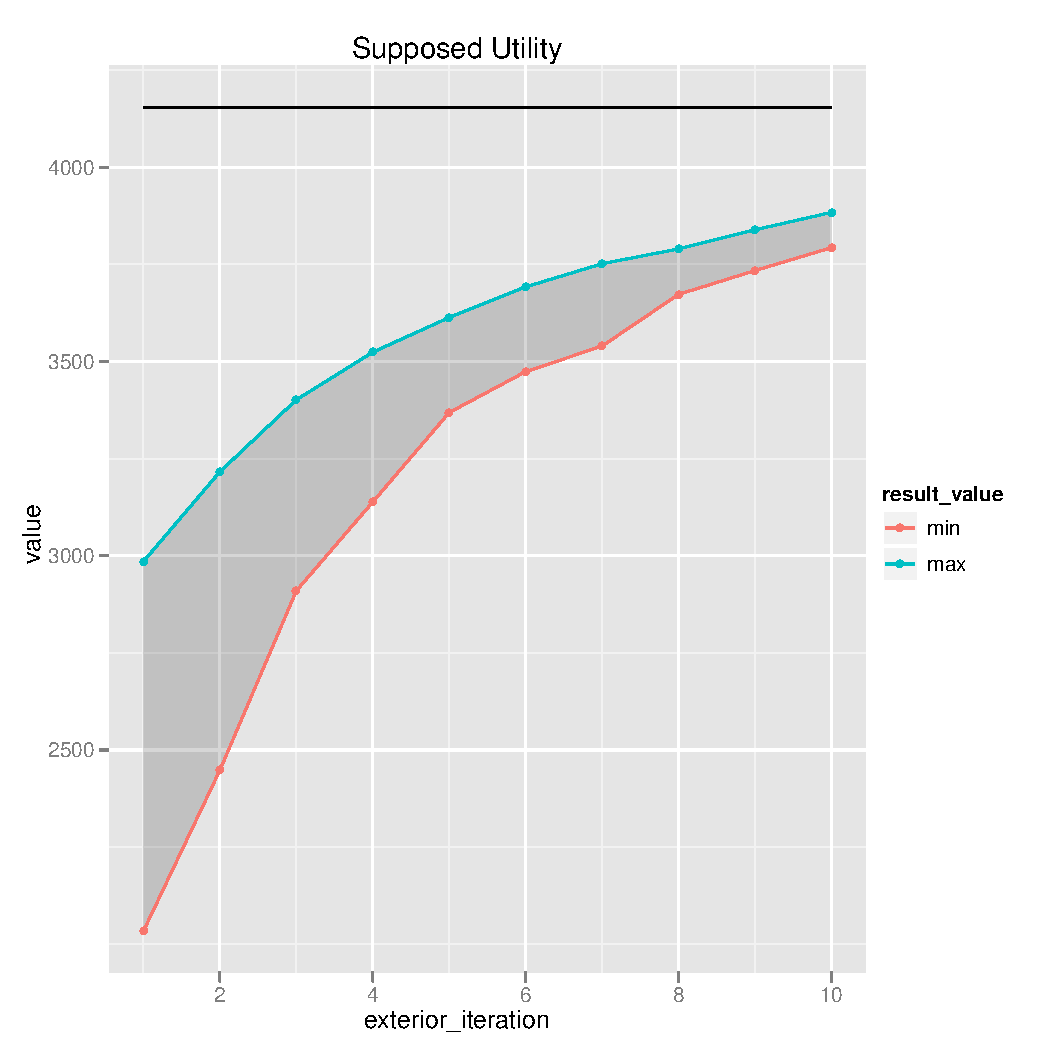
\includegraphics[width=1.0\textwidth]{exp/nouncert/c2_utilouter}
  \caption{Supposed utility function in the exterior loop iterations}
  \label{c2_utilouter}
\end{figure}


%% Utilgen
\begin{figure}
  \centering 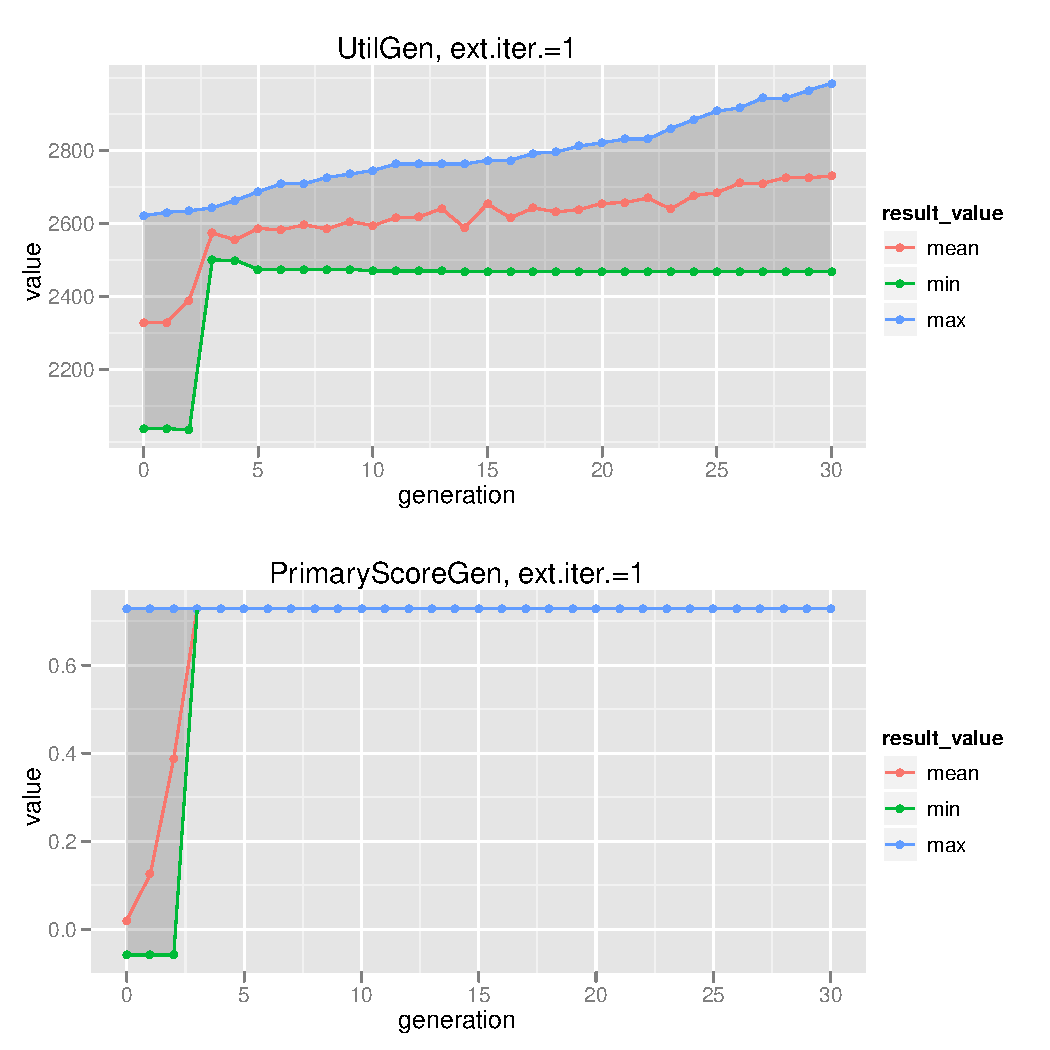
\includegraphics[width=1.0\textwidth]{exp/nouncert/c2_utilgen_01}
  \caption{Supposed utility function in the interior loop iterations}
  \label{c2_utilgen_01}
\end{figure}

\begin{figure}
  \centering 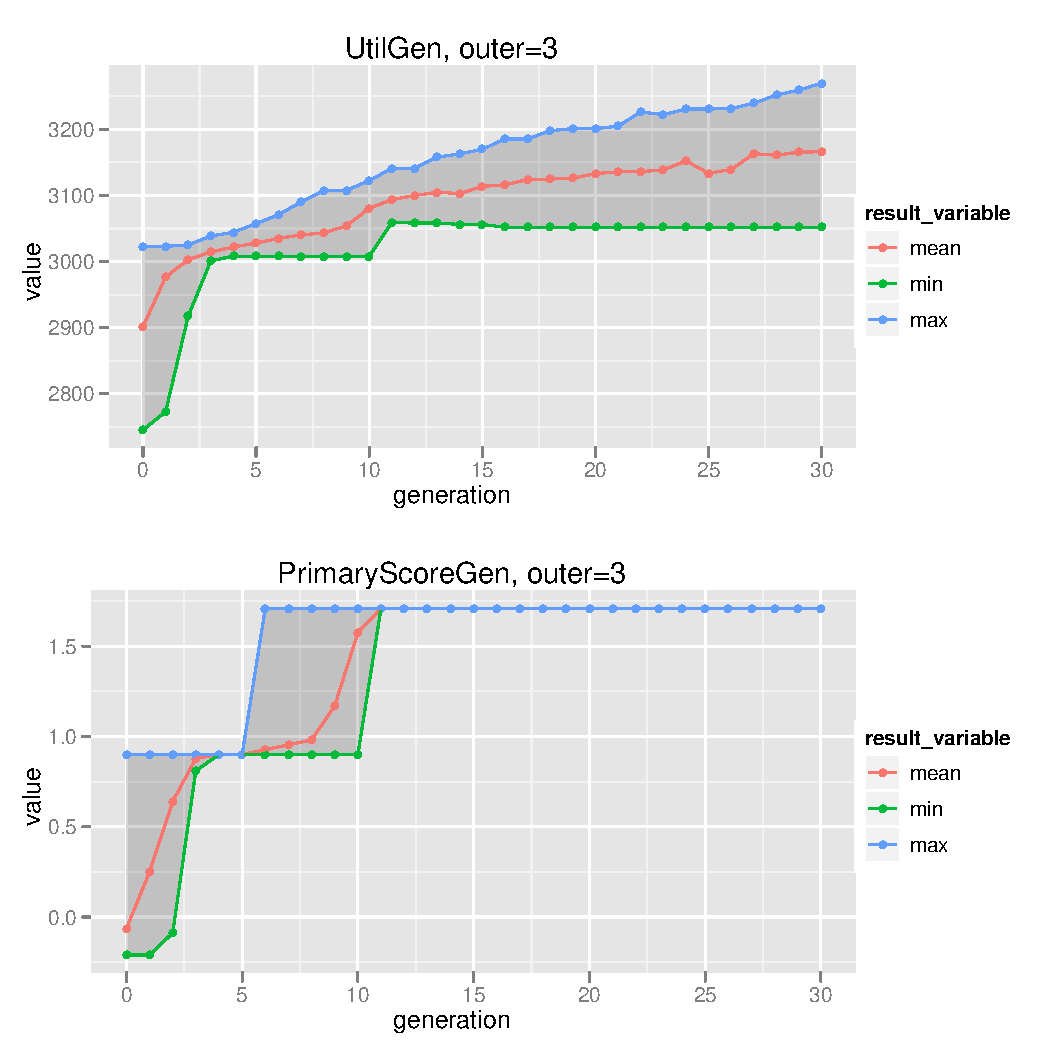
\includegraphics[width=1.0\textwidth]{exp/nouncert/c2_utilgen_03}
  \caption{Supposed utility function in the interior loop iterations}
  \label{c2_utilgen_03}
\end{figure}

\begin{figure}
  \centering 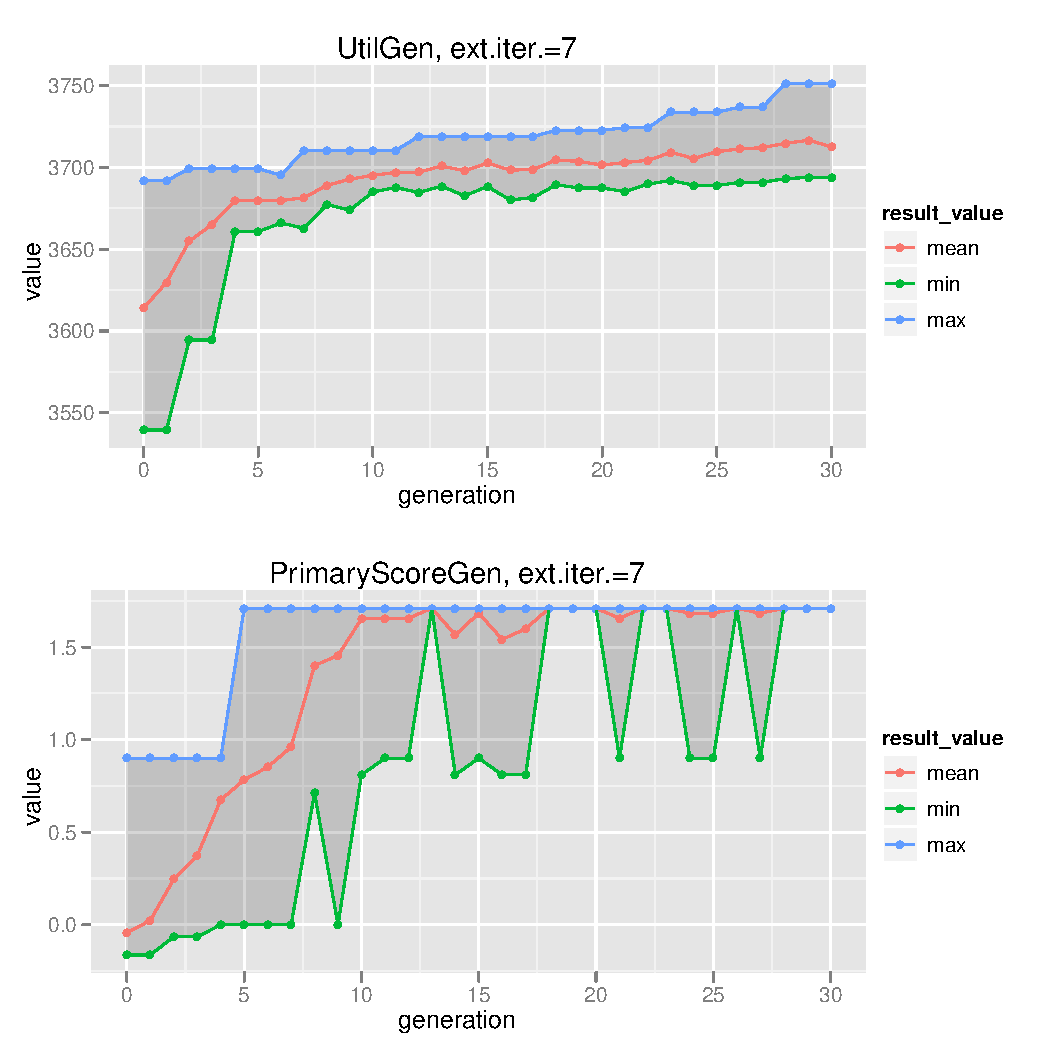
\includegraphics[width=1.0\textwidth]{exp/nouncert/c2_utilgen_07}
  \caption{Supposed utility function in the interior loop iterations}
  \label{c2_utilgen_07}
\end{figure}

%% Valweight
\begin{figure}
  \centering
  \makebox[\textwidth]{
    \subfloat{
      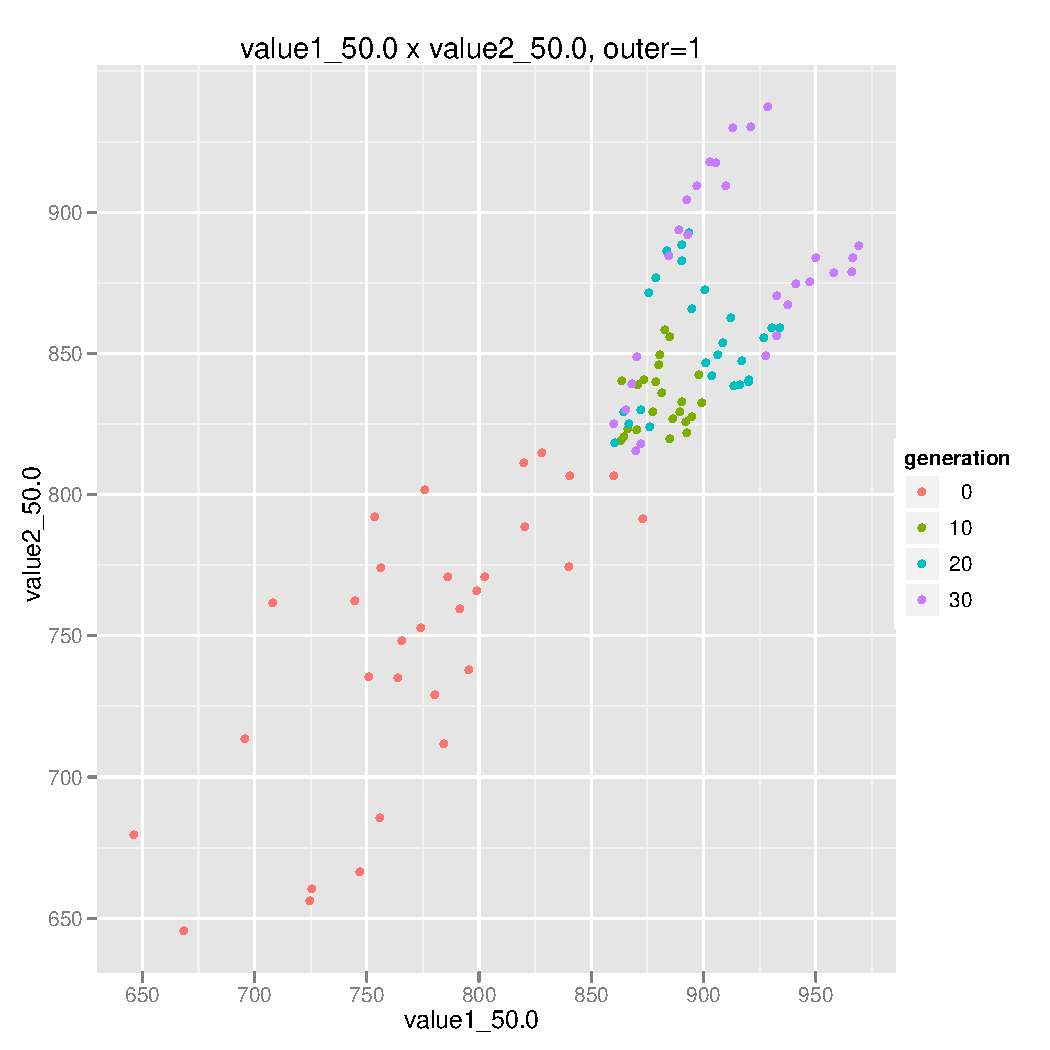
\includegraphics[scale=0.50]{exp/nouncert/c2_valweight_01}
      \label{c2_valweight_01}
    }
    \subfloat{
      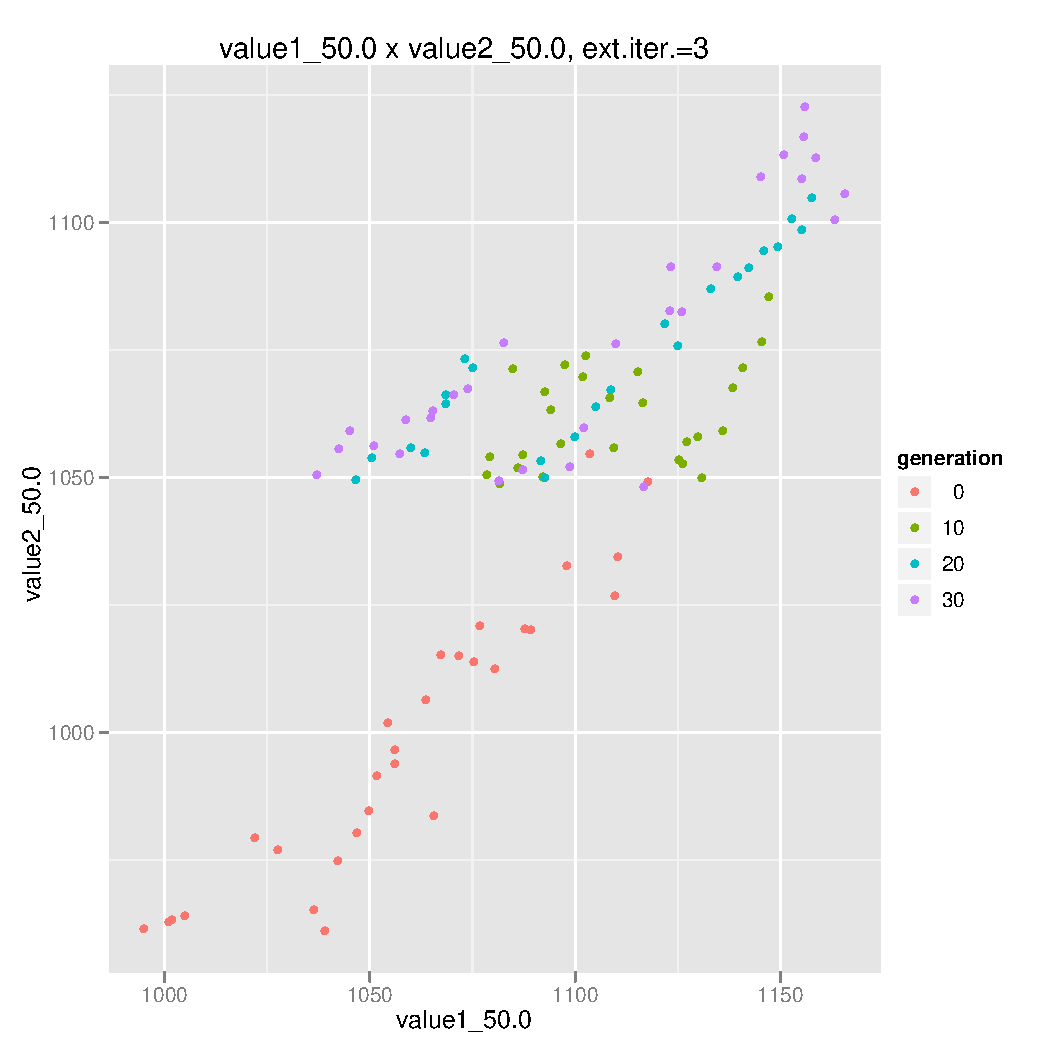
\includegraphics[scale=0.50]{exp/nouncert/c2_valweight_03}
      \label{c2_valweight_03}
    }
  }
  \makebox[\textwidth]{
    \subfloat{
      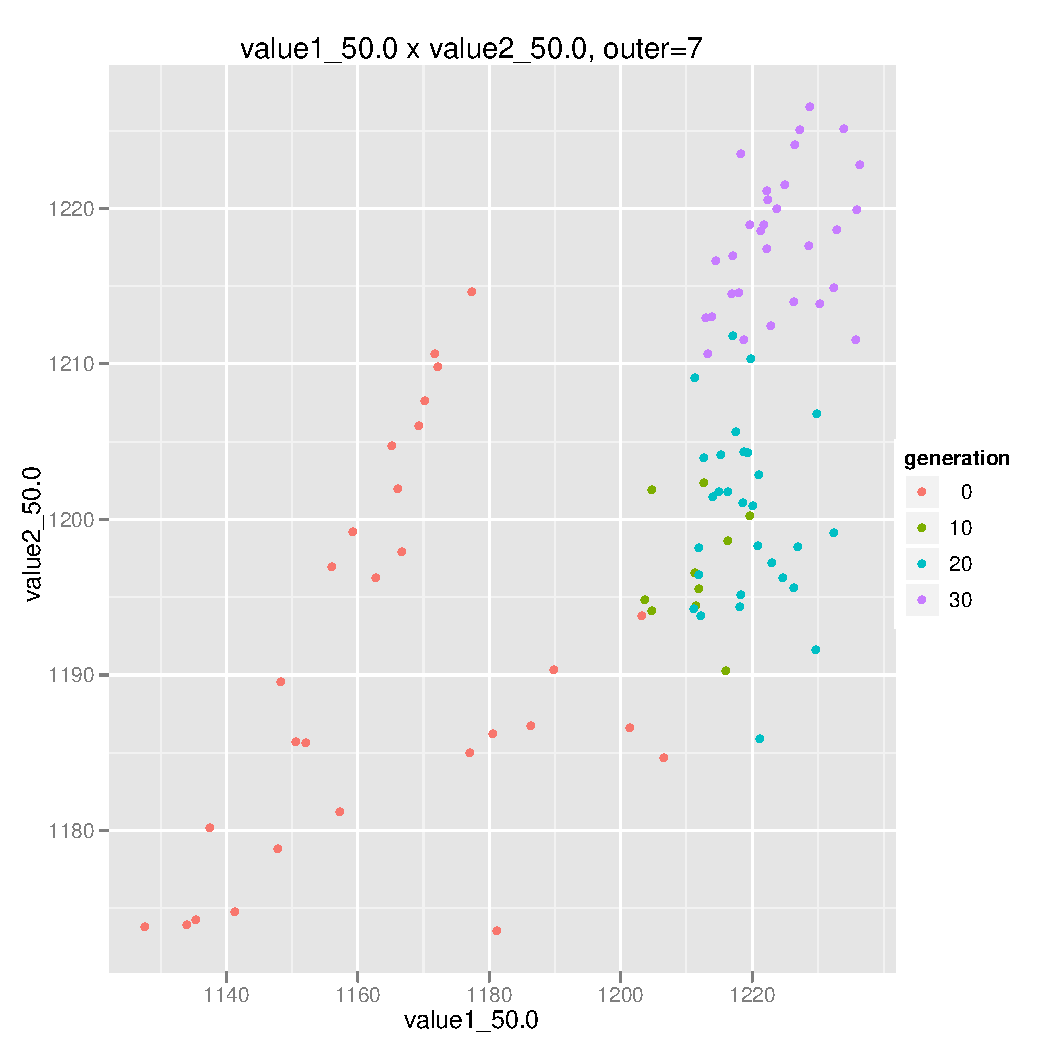
\includegraphics[scale=0.50]{exp/nouncert/c2_valweight_07}
      \label{c2_valweight_07}
    }
  }
  \caption{Individuals in the solution space}
\end{figure}


%% DM's choices
\begin{figure}
  \centering
  \makebox[\textwidth]{
    \subfloat{
      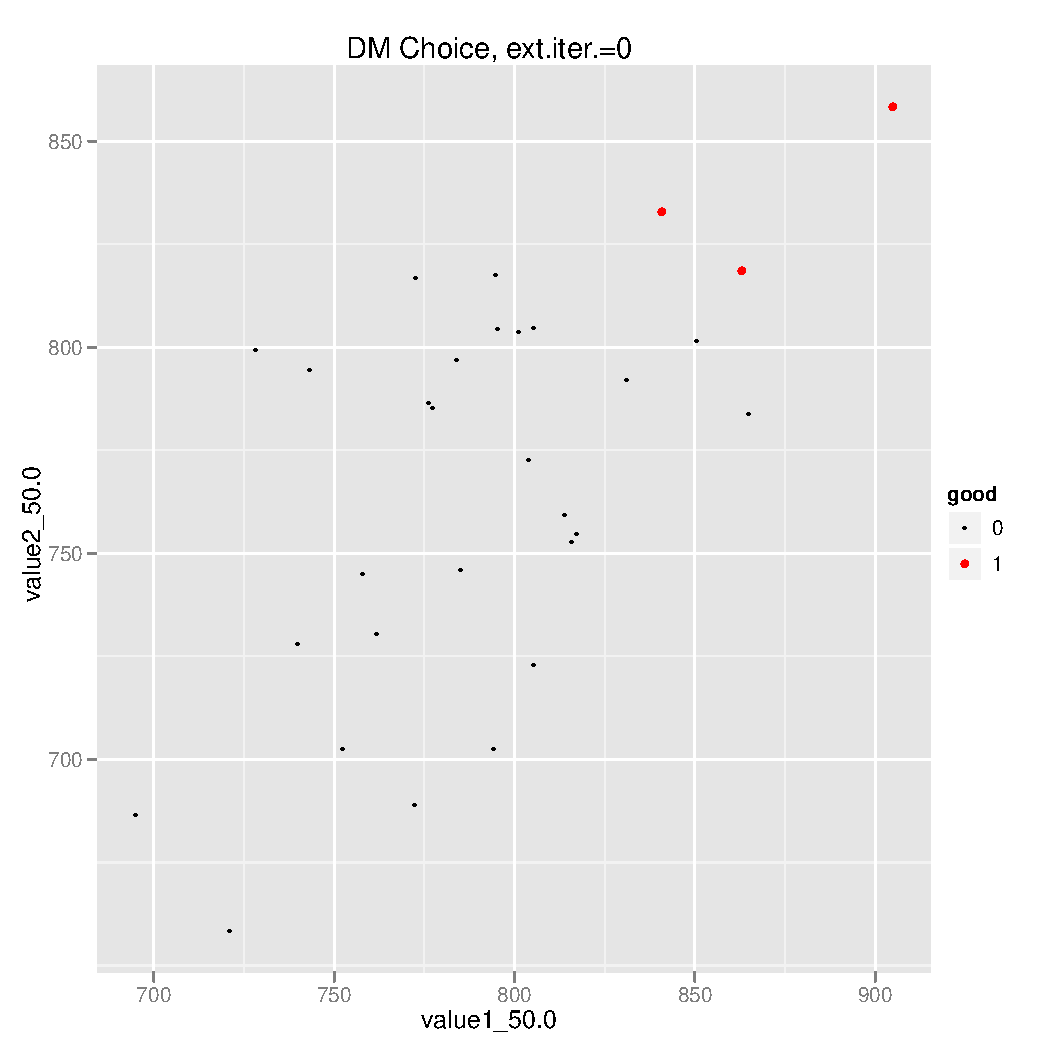
\includegraphics[scale=0.50]{exp/nouncert/c2_dmchoices_01}
      \label{c2_dmchoices_01}
    }
    \subfloat{
      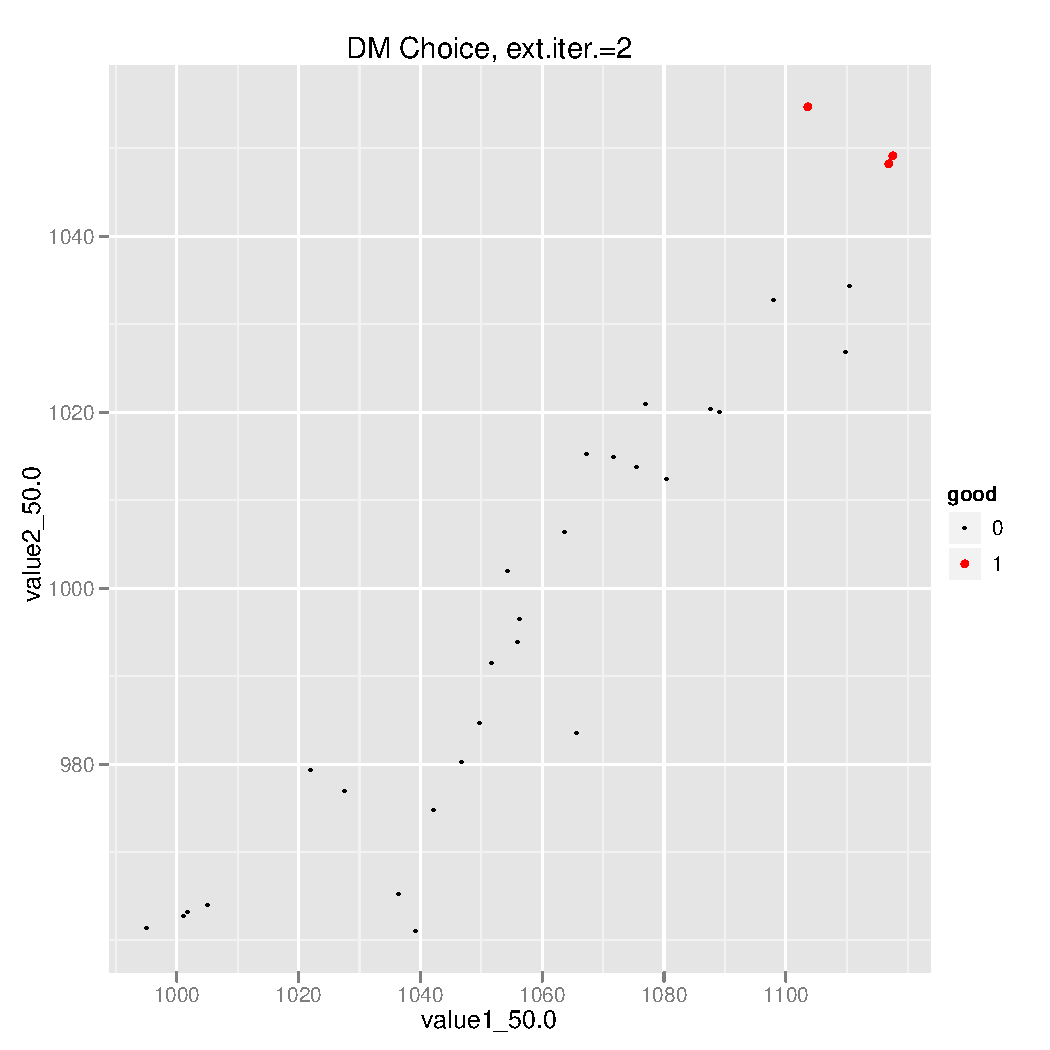
\includegraphics[scale=0.50]{exp/nouncert/c2_dmchoices_03}
      \label{c2_dmchoices_03}
    }
  }
  \makebox[\textwidth]{
    \subfloat{
      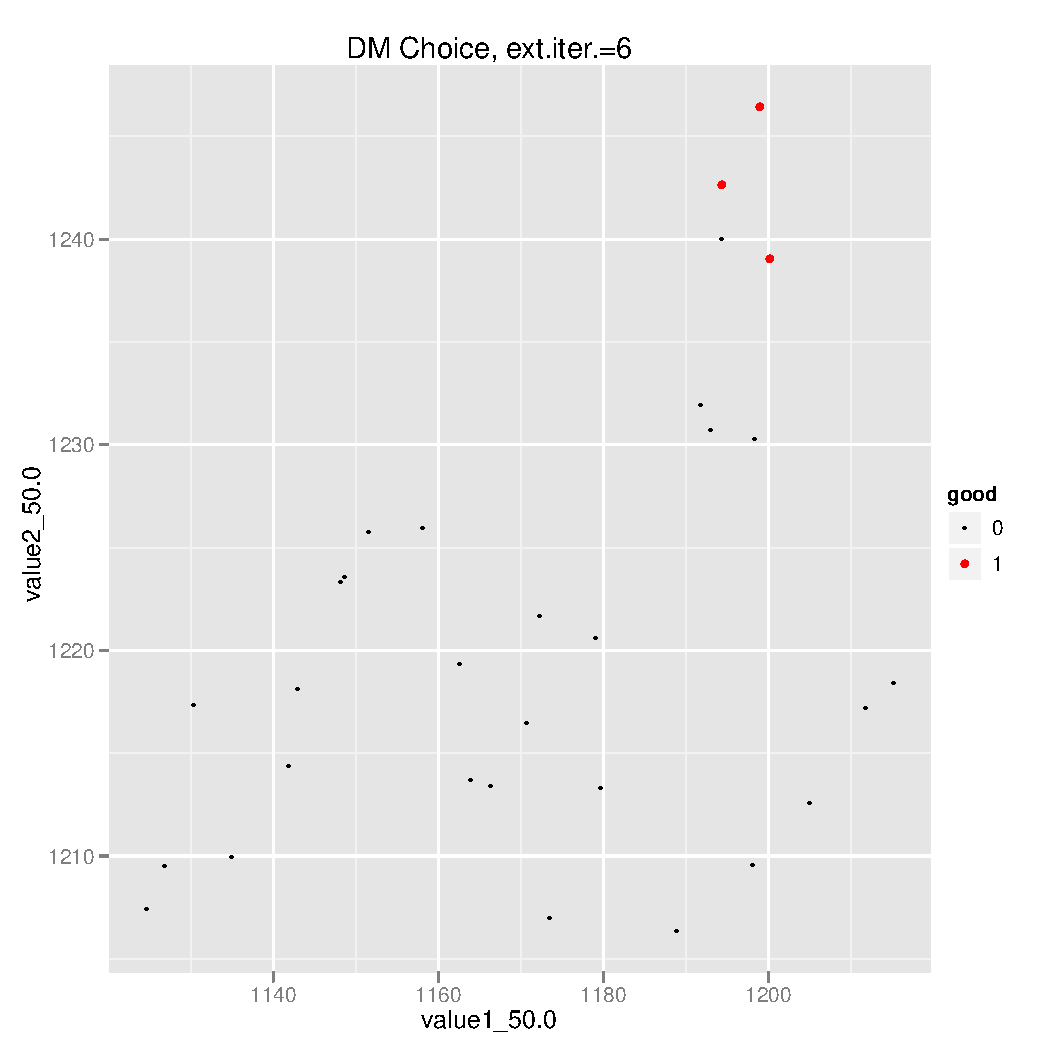
\includegraphics[scale=0.50]{exp/nouncert/c2_dmchoices_07}
      \label{c2_dmchoices_07}
    }
  }
  \caption{Choices made by the DM in exterior loop}
\end{figure}


%% Utilind
\begin{figure}
  \centering 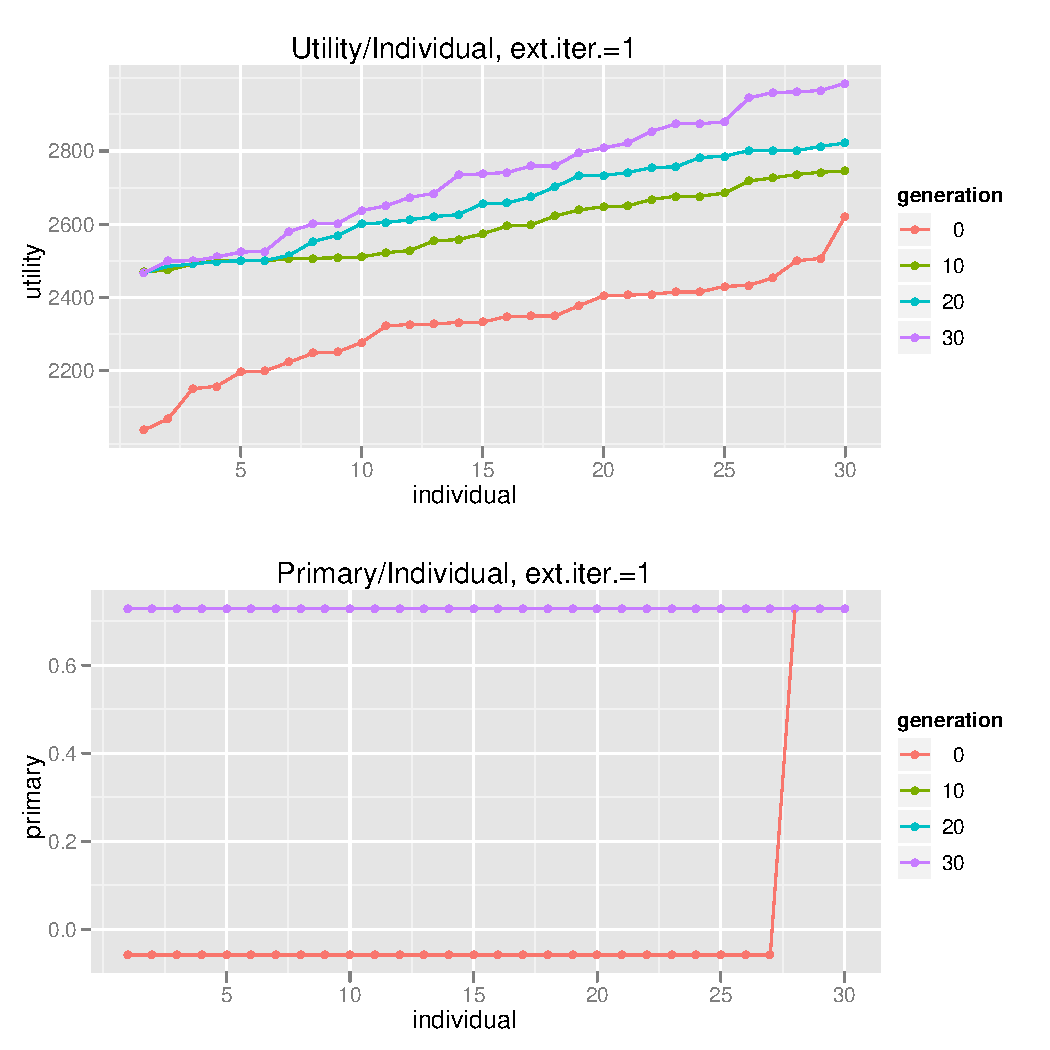
\includegraphics[width=1.0\textwidth]{exp/nouncert/c2_utilind_01}
  \caption{Population advancing through the generations of interior loop}
  \label{c2_utilind_01}
\end{figure}

\begin{figure}
  \centering 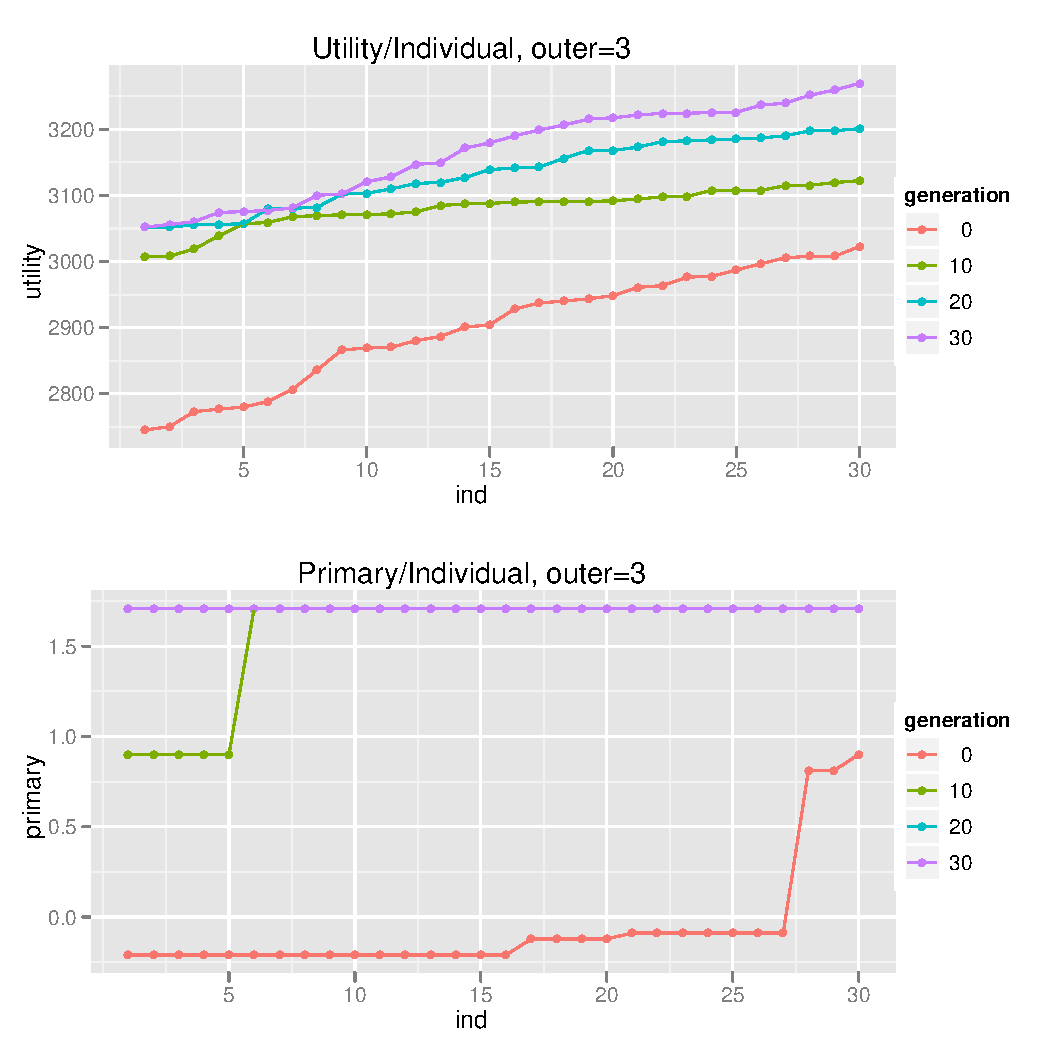
\includegraphics[width=1.0\textwidth]{exp/nouncert/c2_utilind_03}
  \caption{Population advancing through the generations of interior loop}
  \label{c2_utilind_03}
\end{figure}

\begin{figure}
  \centering 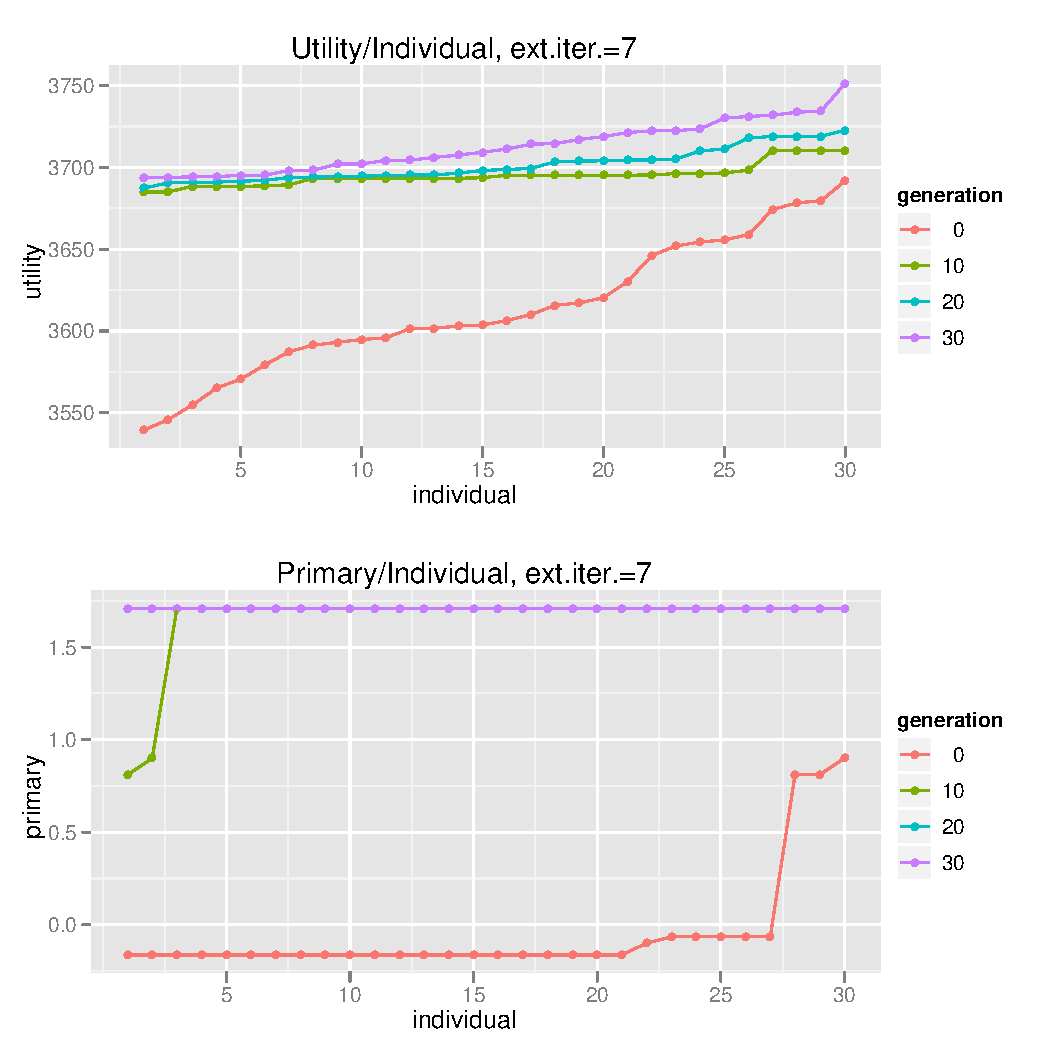
\includegraphics[width=1.0\textwidth]{exp/nouncert/c2_utilind_07}
  \caption{Population advancing through the generations of interior loop}
  \label{c2_utilind_07}
\end{figure}


\clearpage{}
\subsection{The performance on exemplary problems}
\label{nouncert-performance}
It is important to know what performance can be expected from an
algorithm. When no uncertainty is considered in a problem and one assumes the
supposed utility function, then it is easy to get the optimal solution using
linear programming solver. Of course in real-world applications the supposed
utility function is not known a priori. One can test this algorithm in such an
artificially created environment and then assume that the behavior will
resemble the one in real-world problems.

Results of the evaluation on the following problems are given (see~[inref]):
\begin{itemize}
\item Two-criteria binary knapsack problem, optimal value $= 4154.441453$.
\item Two-criteria continuous knapsack problem, optimal value $= 32700.41689$.
\item Three-criteria binary knapsack problem, optimal value $= 31502.10927$.
\item Three-criteria DTLZ problem generated using constraint surface approach, optimal value $= -1.1$.
\end{itemize}

The tests were repeated at least fifteen times and the results averaged. They
are presented in figure~\ref{simple_performance} and
table~\ref{t:opt_dist}. Depending on a problem $10$ or $20$ iterations of the
exterior loop were simulated. Normally it would be up to the DM to stop when
he or she is satisfied with the solution. However, one can safely assume that
if no satisfactory solution is found up to the $10$th iteration, the decision
maker will not want to investigate the problem with this method any further.

\begin{figure}
  \centering
  \makebox[\textwidth]{
    \subfloat{
      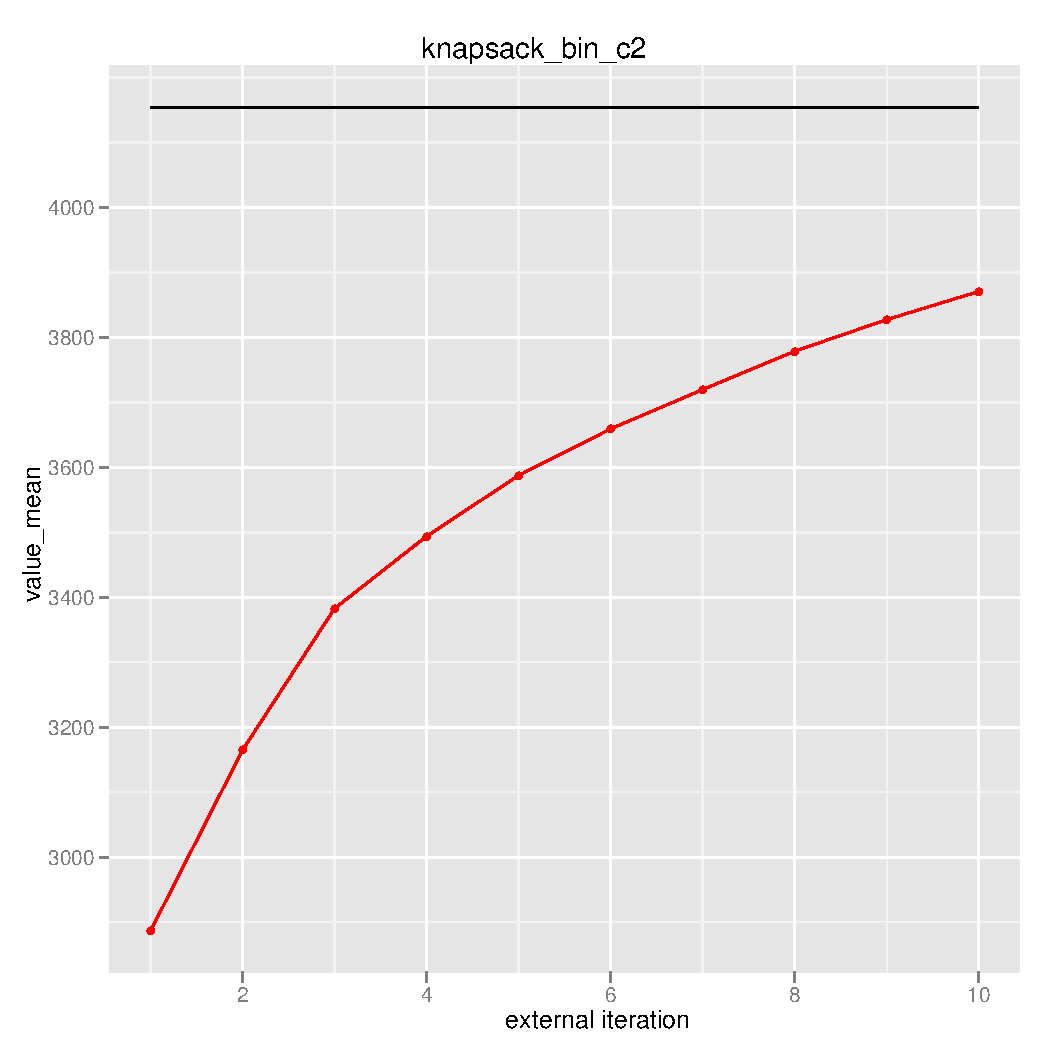
\includegraphics[scale=0.50]{exp/nouncert/c2_knapsack_bin}
      \label{simple_performance1}
    }
    \subfloat{
      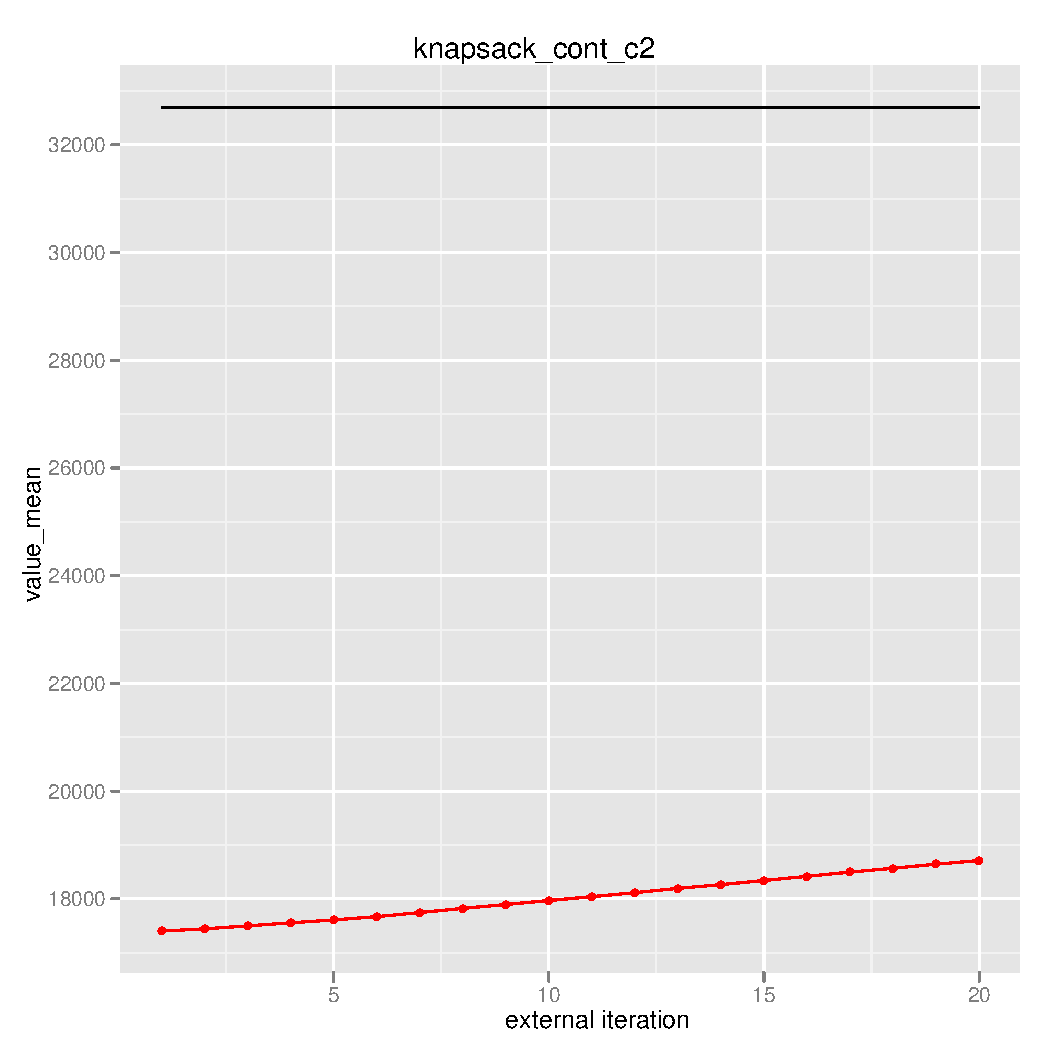
\includegraphics[scale=0.50]{exp/nouncert/c2_knapsack_cont}
      \label{simple_performance2}
    }
  }
  \makebox[\textwidth]{
    \subfloat{
      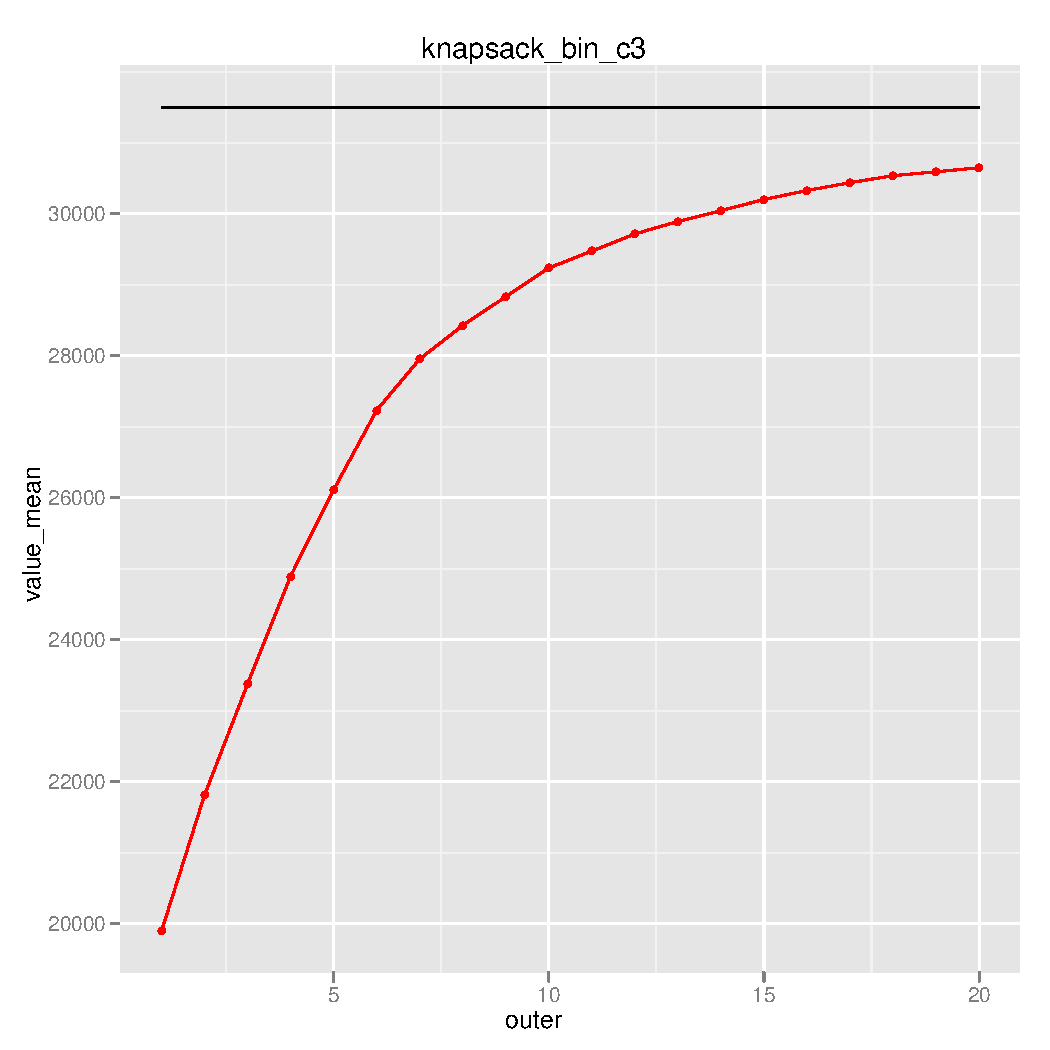
\includegraphics[scale=0.50]{exp/nouncert/c3_knapsack_bin}
      \label{simple_performance3}
    }
    \subfloat{
      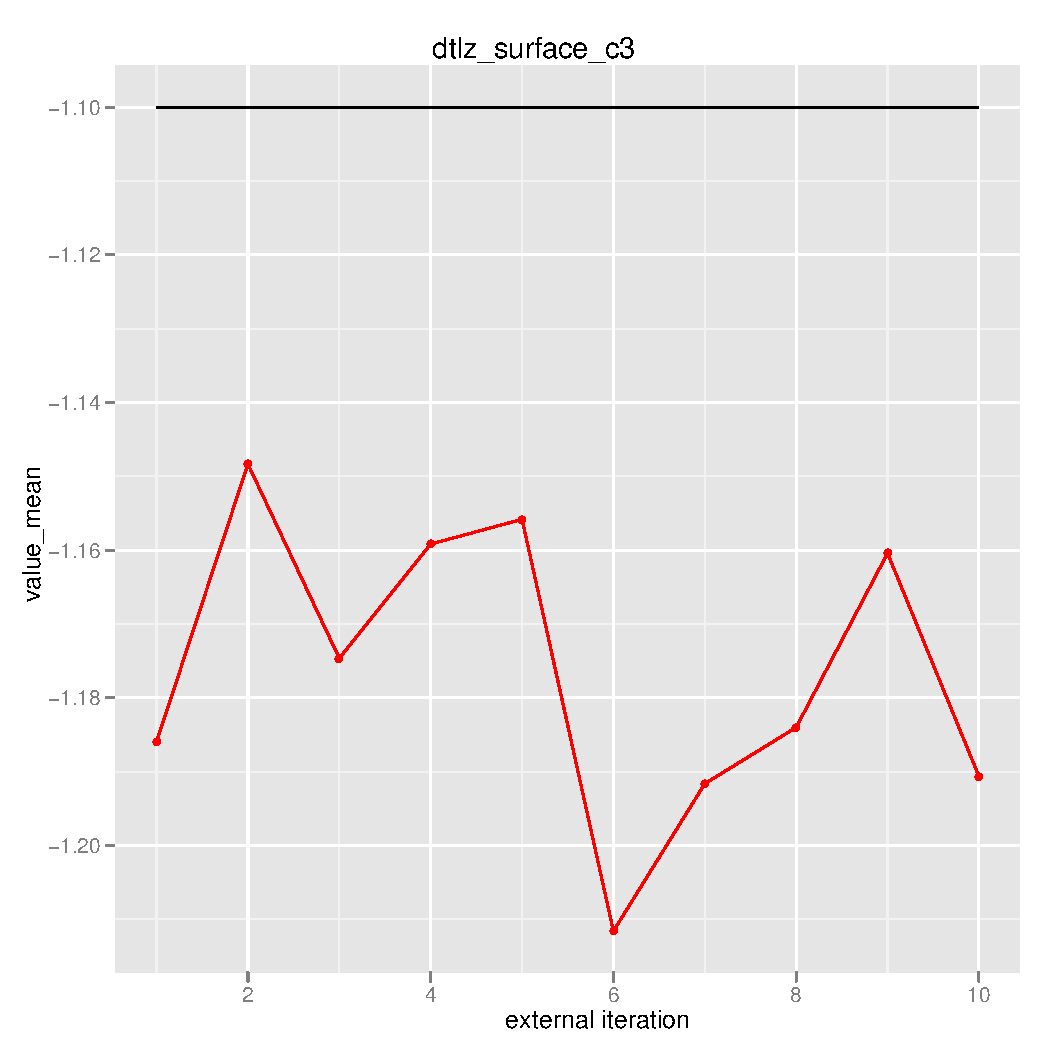
\includegraphics[scale=0.50]{exp/nouncert/c3_surface}
      \label{simple_performance4}
    }
  }
  \caption{Performance comparison}
  \label{simple_performance}
\end{figure}

\begin{table}
  \centering
  \caption{Distance from the optimum solution}
  \label{t:opt_dist}
  \begin{tabular}{r c c c c}
    \hline
    Exterior loop & Knapsack bin 2c & Knapsack cont 2c & Knapsack bin 3c &
    DTLZ surface 3c \\
    \hline
    \hline
    1. & 30.52\% & 46.79\% & 36.85\% & 7.82\% \\
    2. & 23.84\% & 46.66\% & 30.77\% & 4.40\% \\
    3. & 18.61\% & 46.49\% & 25.80\% & 6.79\% \\
    4. & 15.96\% & 46.32\% & 20.99\% & 5.38\% \\
    5. & 13.73\% & 46.16\% & 17.12\% & 5.08\% \\
    6. & 12.02\% & 45.97\% & 13.57\% & 10.15\% \\
    7. & 10.59\% & 45.74\% & 11.28\% & 8.33\% \\
    8. & 9.20\% & 45.51\% & 9.78\% & 7.64\% \\
    9. & 8.05\% & 45.29\% & 8.50\% & 5.49\% \\
    10. & 7.03\% & 45.06\% & 7.22\% & 8.24\% \\
    11. & - & 44.85\% & 6.47\% & - \\
    12. & - & 44.62\% & 5.70\% & - \\
    13. & - & 44.38\% & 5.15\% & - \\
    14. & - & 44.17\% & 4.67\% & - \\
    15. & - & 43.94\% & 4.17\% & - \\
    16. & - & 43.70\% & 3.77\% & - \\
    17. & - & 43.46\% & 3.43\% & - \\
    18. & - & 43.25\% & 3.12\% & - \\
    19. & - & 43.02\% & 2.94\% & - \\
    20. & - & 42.81\% & 2.77\% & - \\
    \hline
  \end{tabular}
\end{table}

On both binary knapsack problems the performance is very good --- they are not
further than $10\%$ away from the optimal solution after the $10$th
iteration. The same is true for the surface problem. However, looking at the
fig.~\ref{simple_performance4} one can see a bizarre phenomenon --- the
supposed utility is falling down in a few runs.

On the other hand, the evolutionary algorithm knows nothing about the utility
function so it may happen. The chart (fig.~\ref{simple_performance4}) was
generated using aggregated (averaged) results, however this happened in most
of the runs. To give a further insight charts showing evolution in a third
exterior loop are presented (not that the charts are for a single run only,
not aggregated). The charts are in figures~\ref{c3_surface_utilgen_03}
and~\ref{c3_surface_utilind_03}. As one can see the evolutionary algorithm
improves the population from its perspective (the primary score factor).
However, supposed utility function is being lowered in the process.

\begin{figure}
  \centering
  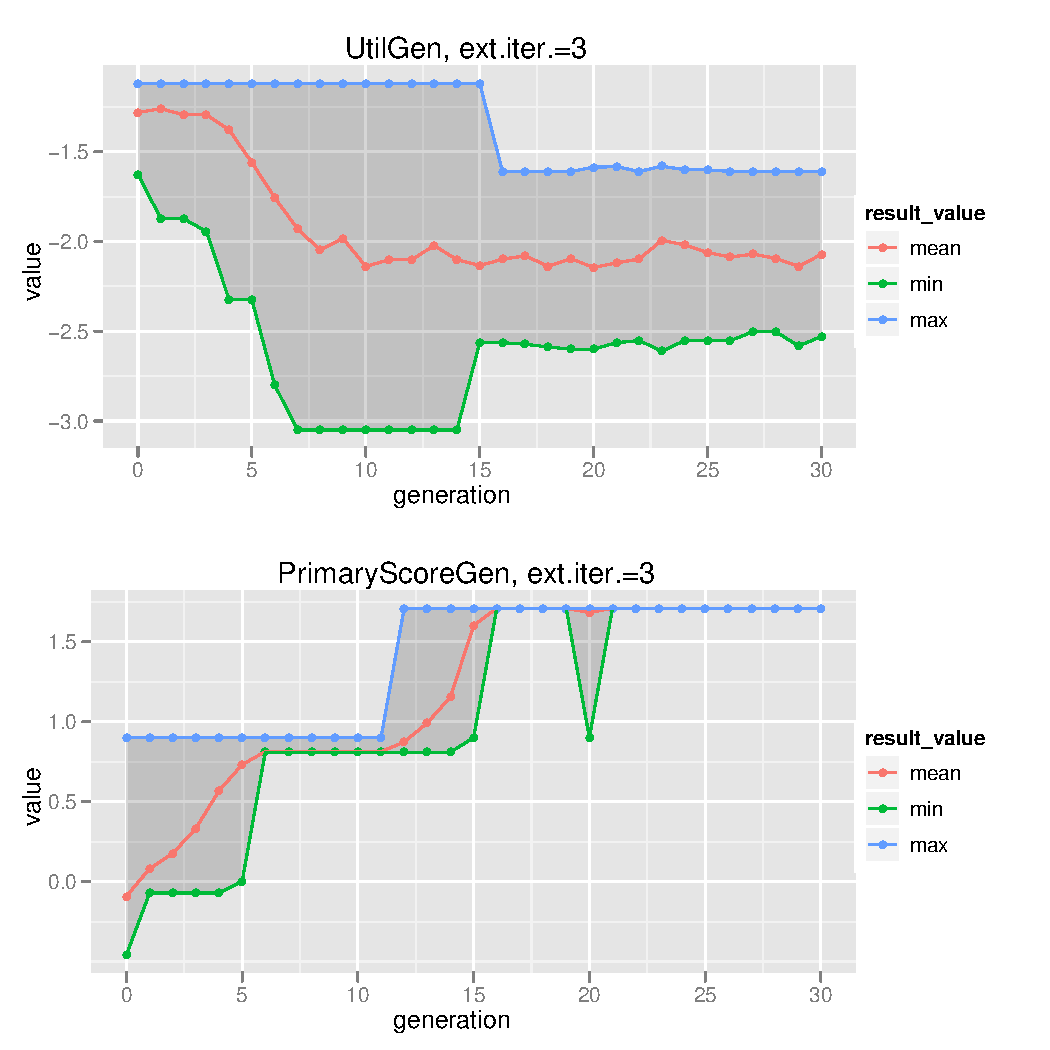
\includegraphics[width=1.0\textwidth]{exp/nouncert/c3_surface_utilgen_03}
  \caption{The population in the third iteration of the exterior loop. DTLZ
    surface problem.}
  \label{c3_surface_utilgen_03}
\end{figure}

\begin{figure}
  \centering
  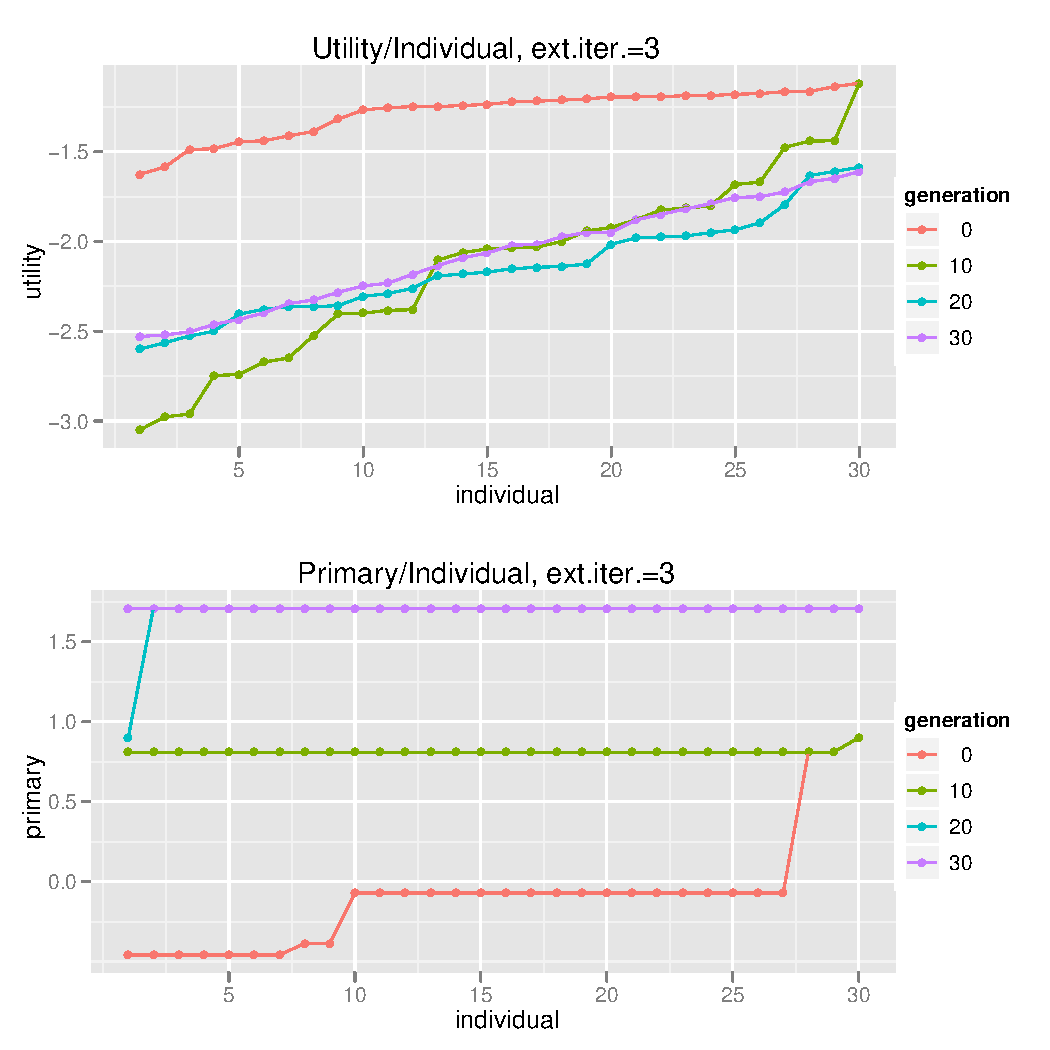
\includegraphics[width=1.0\textwidth]{exp/nouncert/c3_surface_utilind_03}
  \caption{The population in the third iteration of the exterior loop. DTLZ
    surface problem}
  \label{c3_surface_utilind_03}
\end{figure}

This is the case because generated decision rules:
\begin{enumerate}
\item $f_1 \le 0.14033 \Rightarrow \text{class} \ge \texttt{GOOD}$
\item $f_3 \le 0.56462 \Rightarrow \text{class} \ge \texttt{GOOD}$
\end{enumerate}
are not selective enough. It is possible that switching DomLem to another
algorithm --- generating all possible rules instead of a minimal set would
help here. Still the results achieved by the DARWIN method are good on this
problem.

On the contrary, continuous knapsack problem performs extremely poor --- only
$55\%$ of the optimum after the $10$th run and $58\%$, so almost no
improvement, after the $20$th. Investigating single runs at length provided no
more details. The problem lies in the evolutionary algorithm, more precisely
in its crossover operator. In the DARWIN method a from of the distance
preserving crossover is used. The form where a child is somewhere in between
its parents. However, in continuous variant it is usually the case to take
items one-by-one starting with the one with the greatest value per unit until
the weight constraint is reached.

Considering the constraints ($ \forall_{x_i \in items}: \hspace{0.1cm} 0 \leq
x_i \leq 1 $) --- most of the individuals will have their decision variables
in the form of $x_i \approx 0.5$ after a few generations. But for the optimal
solutions most of the variables take either $1$ or $0$. That is why
improvement is happening so slowly here.

Relying on the author's intuition changing the crossover operator would solve
the problem with continuous knapsack. Choosing the right operator for a given
problem is a well-known subject in the multi-objective optimization
([ref]). However, it is out-of-scope of this paper.

For completeness charts presenting the algorithm behavior when more exterior
loop iterations are allowed are given (fig.~\ref{outer},
table~\ref{t:opt_dist_long}). After the twentieth loop improvements are small
(if any). In author's opinion this is a good thing because there is no reason
not to stop the algorithm. If the algorithm works well on a problem it will be
evident from the first few iterations.

\begin{figure}
  \centering
  \makebox[\textwidth]{
    \subfloat{
      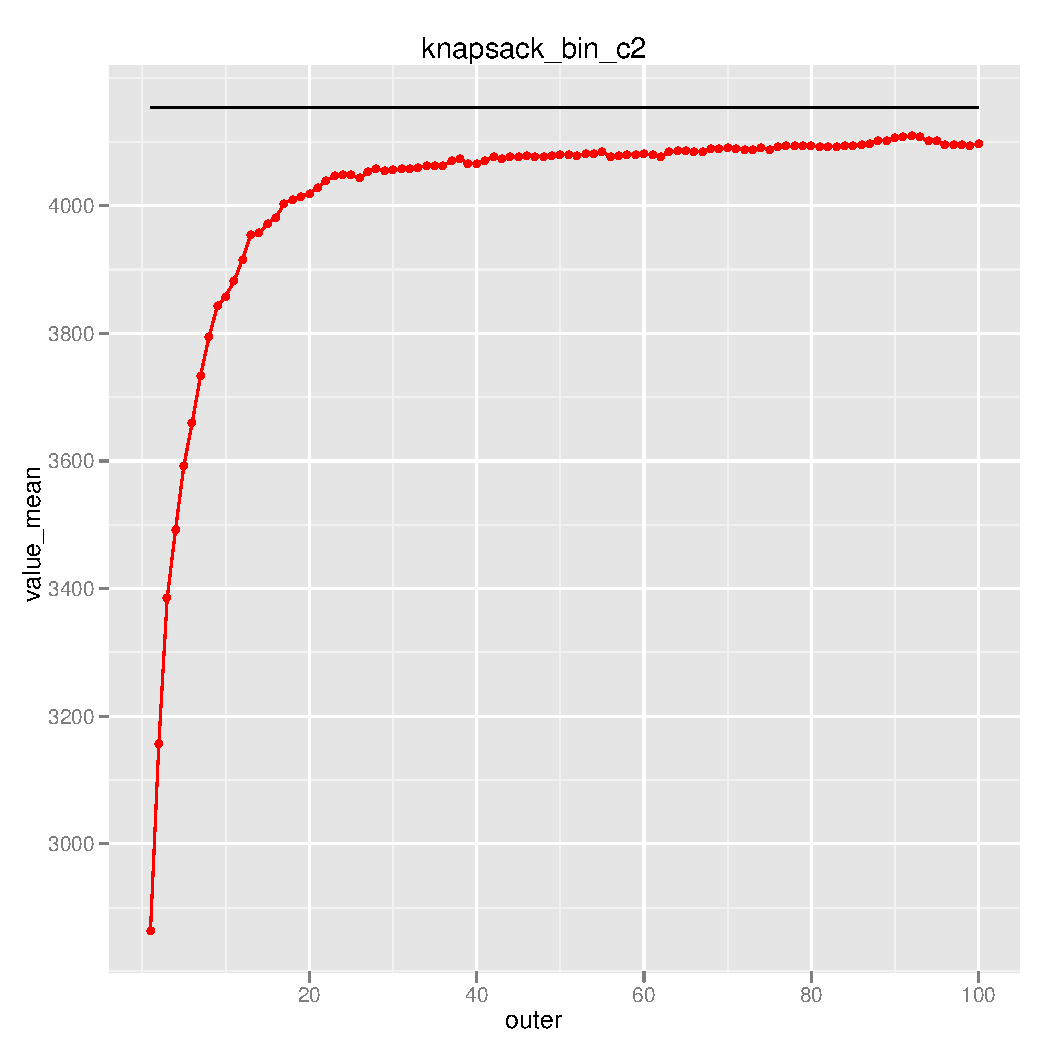
\includegraphics[scale=0.50]{exp/nouncert/c2_knapsack_bin_outer}
      \label{outer1}
    }
    \subfloat[TODO!]{
      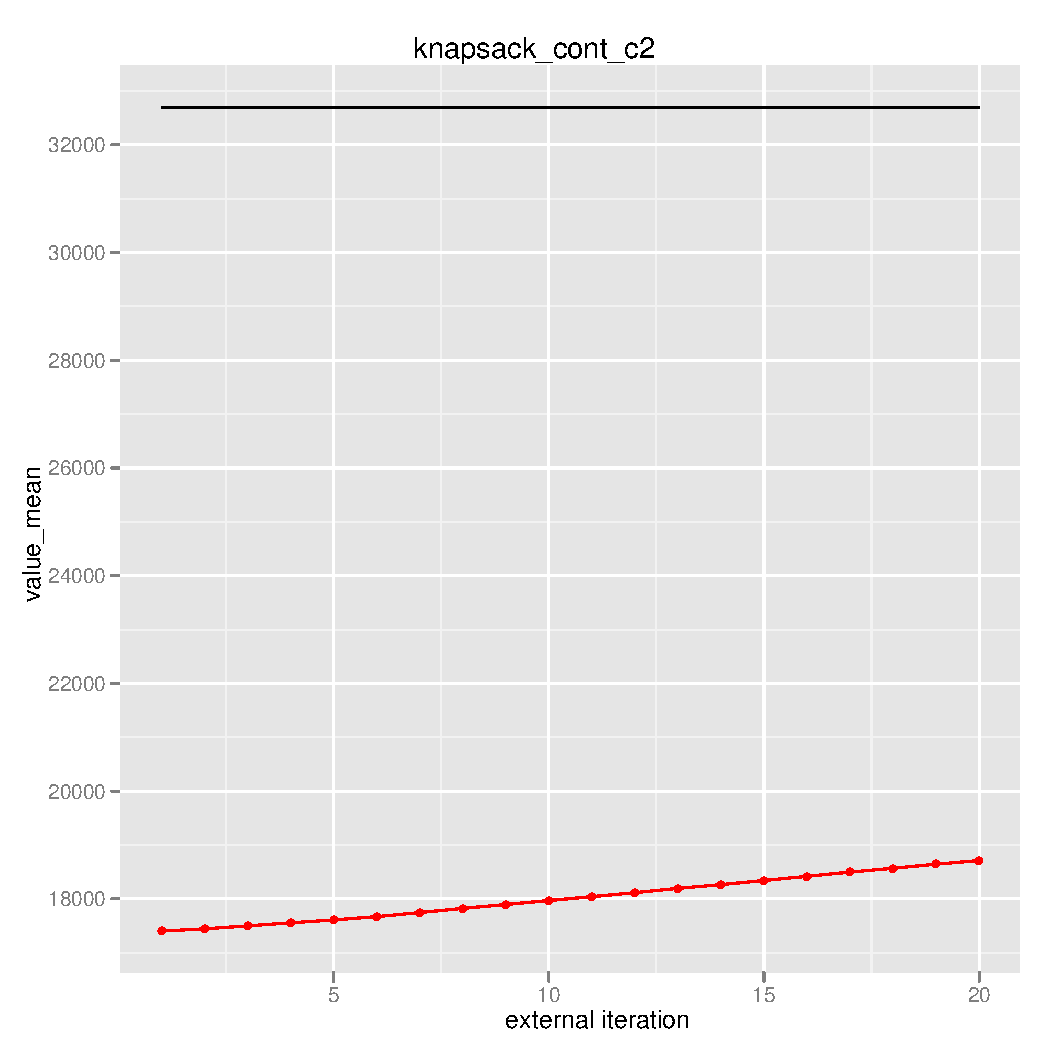
\includegraphics[scale=0.50]{exp/nouncert/c2_knapsack_cont}
      \label{outer2}
    }
  }
  \makebox[\textwidth]{
    \subfloat{
      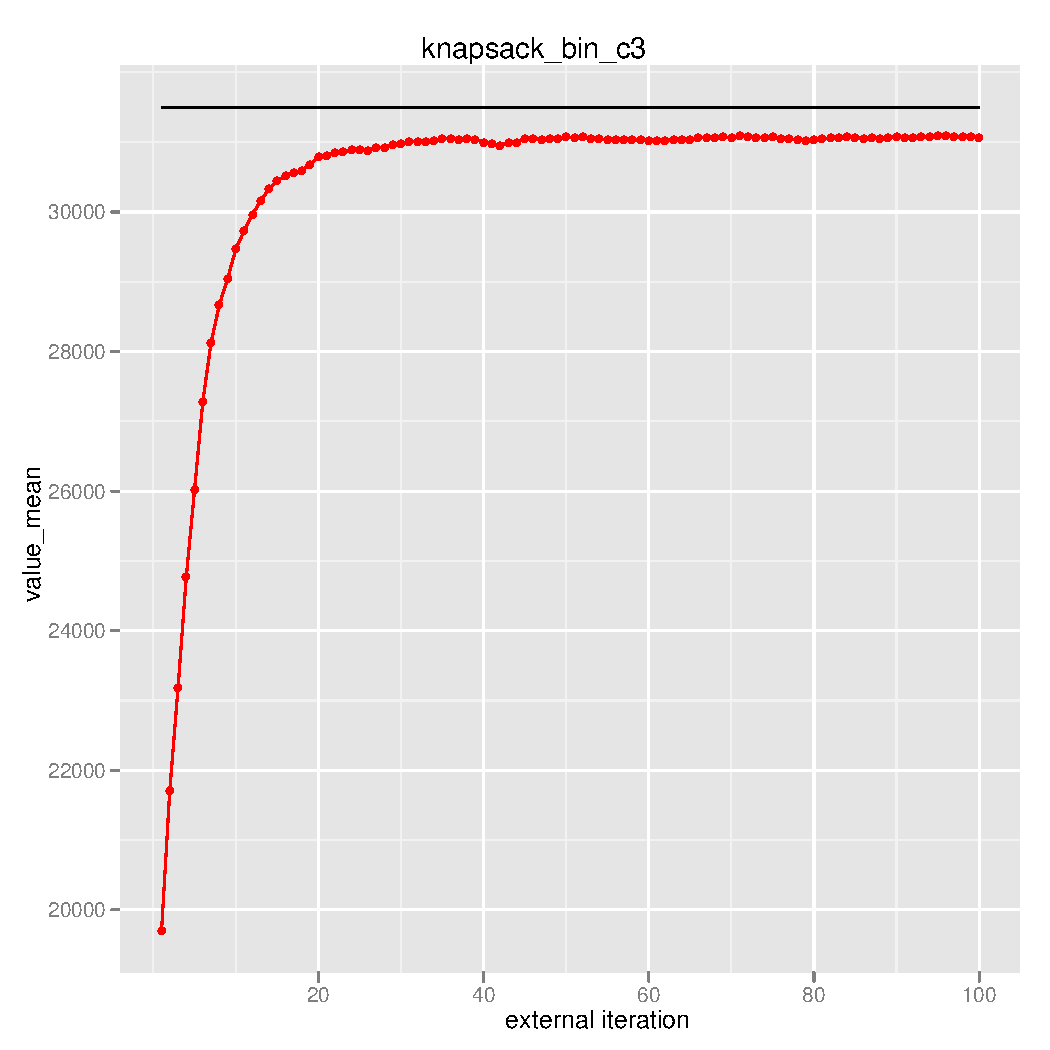
\includegraphics[scale=0.50]{exp/nouncert/c3_knapsack_bin_outer}
      \label{outer3}
    }
    \subfloat{
      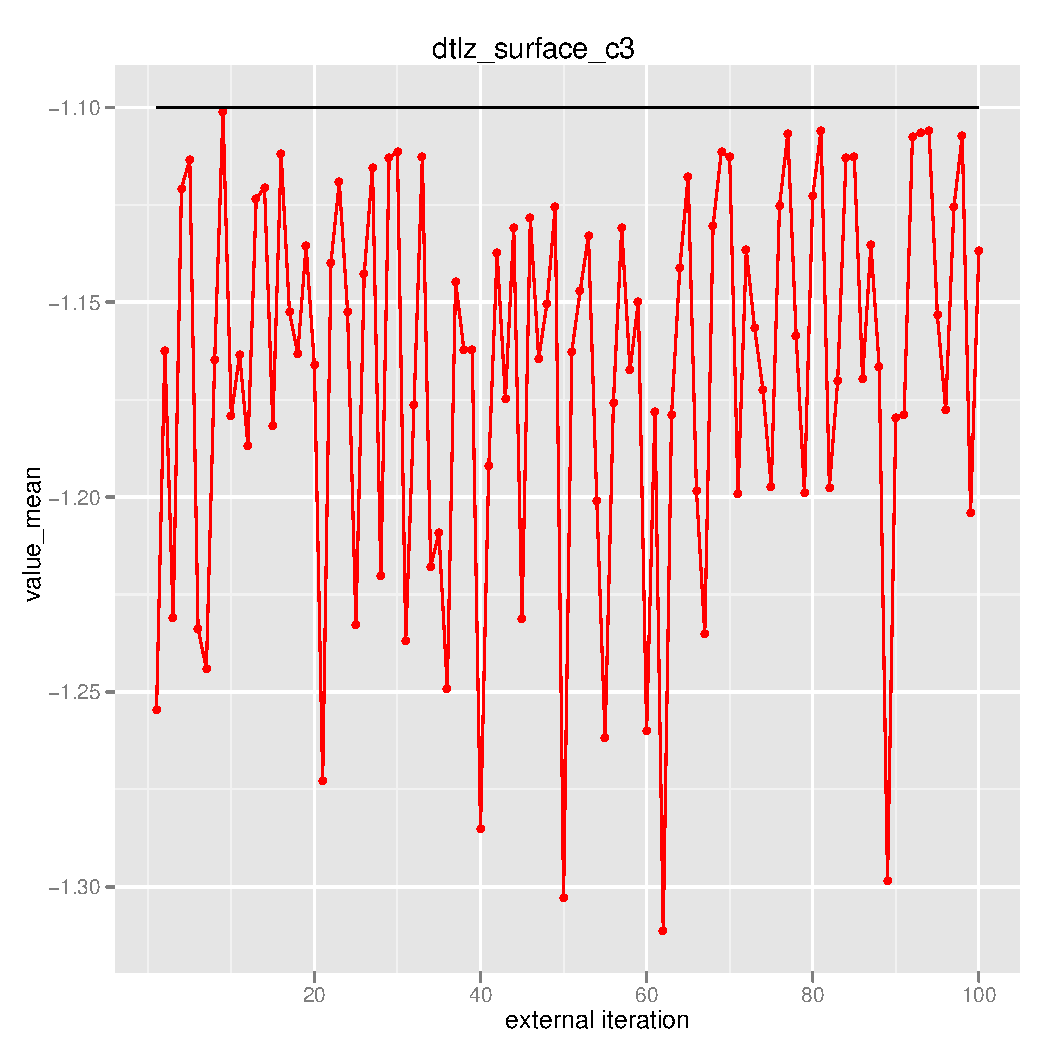
\includegraphics[scale=0.50]{exp/nouncert/c3_surface_outer}
      \label{outer4}
    }
  }
  \caption{Supposed utility function when long runs are allowed}
  \label{outer}
\end{figure}

\begin{table}
  \centering
  \caption{Distance from the optimum solution when long runs are allowed}
  \label{t:opt_dist_long}
  \begin{tabular}{r c c c c}
    \hline
    Exterior loop & Knapsack bin 2c & Knapsack cont 2c & Knapsack bin 3c &
    DTLZ surface 3c \\
    \hline
    \hline
    1 & 31.08\% & TODO & 37.48\% & 14.05\% \\
    5 & 13.59\% & TODO & 17.42\% & 1.22\% \\
    10 & 7.33\% & TODO & 6.48\% & 7.19\% \\
    15 & 4.72\% & TODO & 3.39\% & 7.43\% \\
    20 & 3.70\% & TODO & 2.33\% & 6.00\% \\
    25 & 3.11\% & TODO & 2.02\% & 12.06\% \\
    30 & 3.05\% & TODO & 1.75\% & 1.05\% \\
    35 & 2.99\% & TODO & 1.56\% & 9.93\% \\
    40 & 3.05\% & TODO & 1.73\% & 16.83\% \\
    45 & 2.91\% & TODO & 1.58\% & 11.93\% \\
    50 & 2.94\% & TODO & 1.49\% & 18.44\% \\
    55 & 2.94\% & TODO & 1.65\% & 14.70\% \\
    60 & 3.15\% & TODO & 1.70\% & 14.55\% \\
    65 & 3.13\% & TODO & 1.69\% & 1.61\% \\
    70 & 3.14\% & TODO & 1.60\% & 1.16\% \\
    75 & 3.34\% & TODO & 1.60\% & 8.86\% \\
    80 & 3.31\% & TODO & 1.71\% & 2.07\% \\
    85 & 3.41\% & TODO & 1.66\% & 1.15\% \\
    90 & 3.22\% & TODO & 1.62\% & 7.24\% \\
    95 & 3.45\% & TODO & 1.59\% & 4.85\% \\
    100 & 3.66\% & TODO & 1.71\% & 3.34\% \\
    \hline
  \end{tabular}
\end{table}

\clearpage{}
\subsection{The importance of parameters}

The algorithm itself contains many parameters that can potentially affect its
behaviour. Of course it is always left to the analyst to fine-tune the
parameters for a specific problem to solve. Nevertheless in this section some
guidelines will be given. Conclusions were drawn on the basis of experiments
performed on exemplary problems described above.

The parameters were grouped into two categories --- basic ones affecting the
whole method and additional ones of less importance. The latter, however, can
be used for fine-tuning to specific problem given.

The author considers the basic parameters to be:
\begin{itemize}
\item Number of generation in the evolutionary loop --- intuitively the more
  the better.
\item Number of individuals in the population --- again intuitively the more
  the better.
\item A confidence of the rules generated in the DomLem algorithm. (compare
  with~[inref]). 100\% confidence may seem a good idea; however, lowering it
  would allow more gradual improvements of the goal function in the
  evolutionary algorithm which could lead to better results.
\end{itemize}


\begin{figure}
  \centering
  \makebox[\textwidth]{
    \subfloat{
      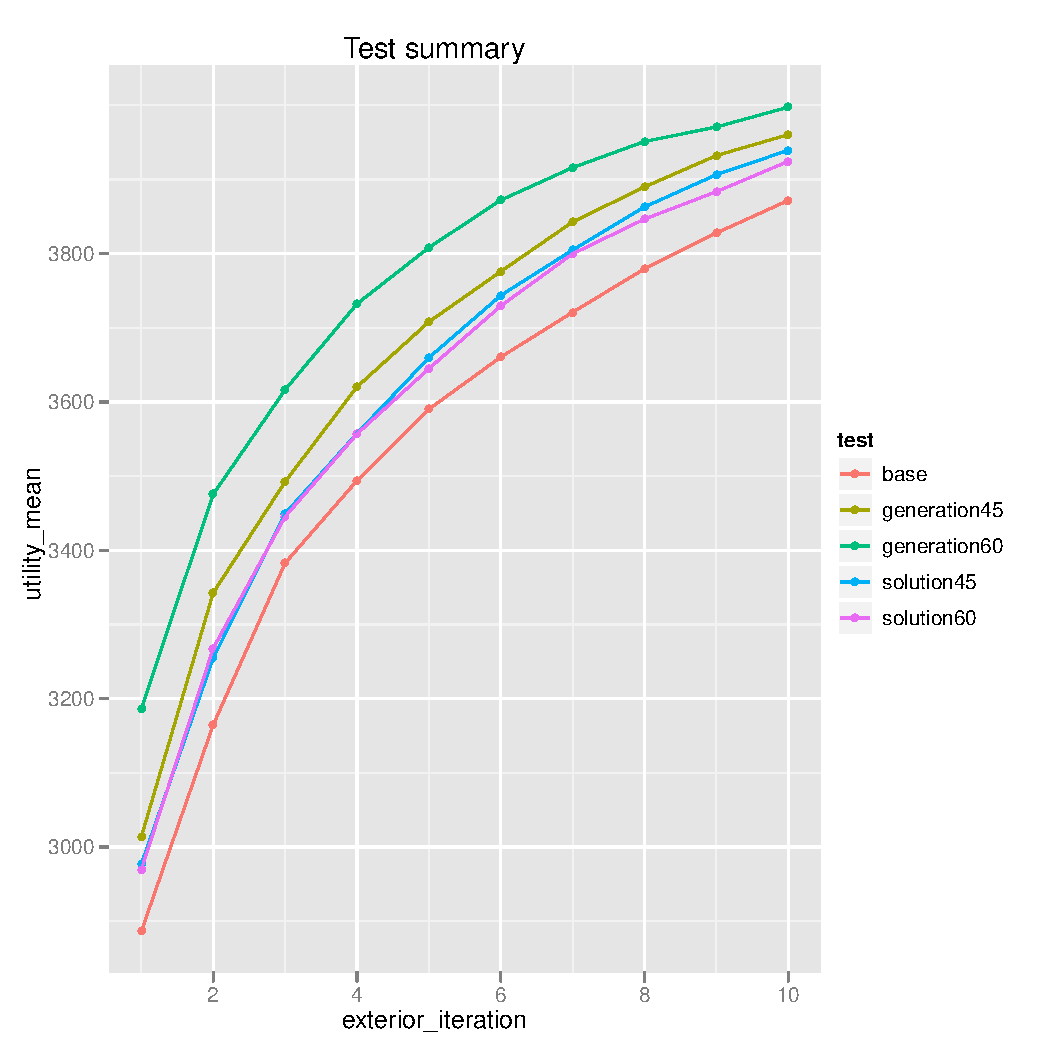
\includegraphics[width=0.65\textwidth]{exp/nouncert/c2_params1}
      \label{c2_params1}
    }
    \subfloat{
      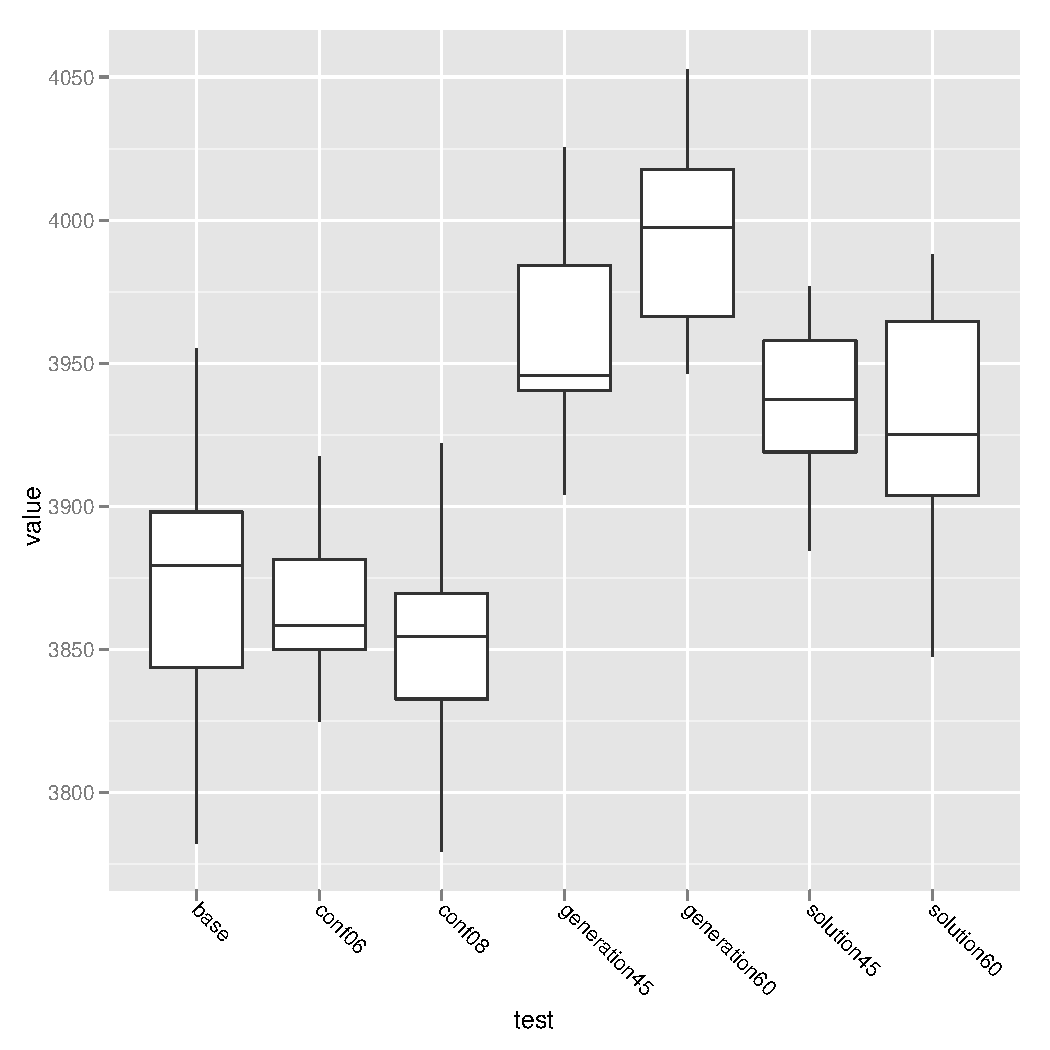
\includegraphics[width=0.65\textwidth]{exp/nouncert/c2_params1b}
      \label{c2_params1b}
    }
  }
  \caption{Basic parameters for the two-criteria binary knapsack problem}
  \label{c2_params}
\end{figure}

\begin{figure}
  \centering
  \makebox[\textwidth]{
    \subfloat{
      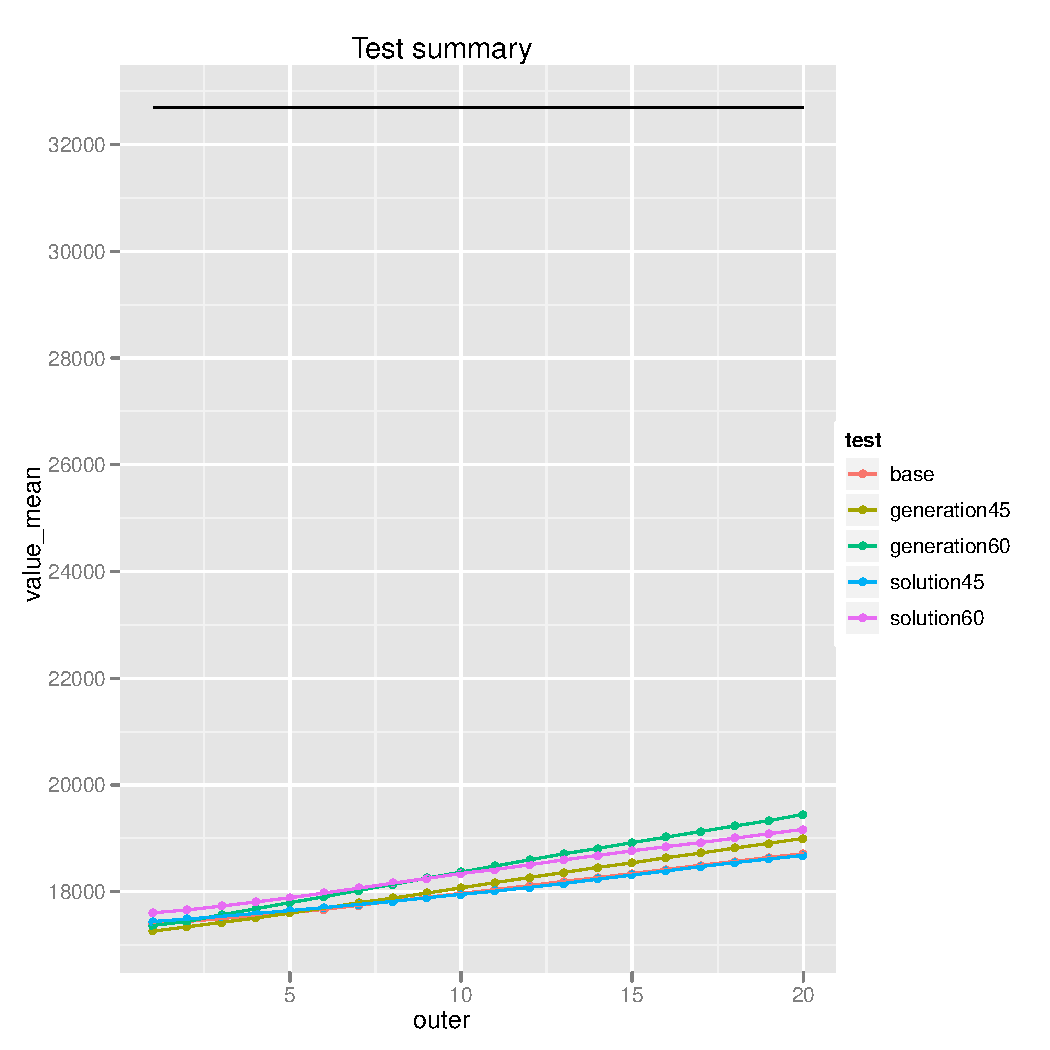
\includegraphics[width=0.65\textwidth]{exp/nouncert/c2_cont_params1}
      \label{c2_cont_params1}
    }
    \subfloat{
      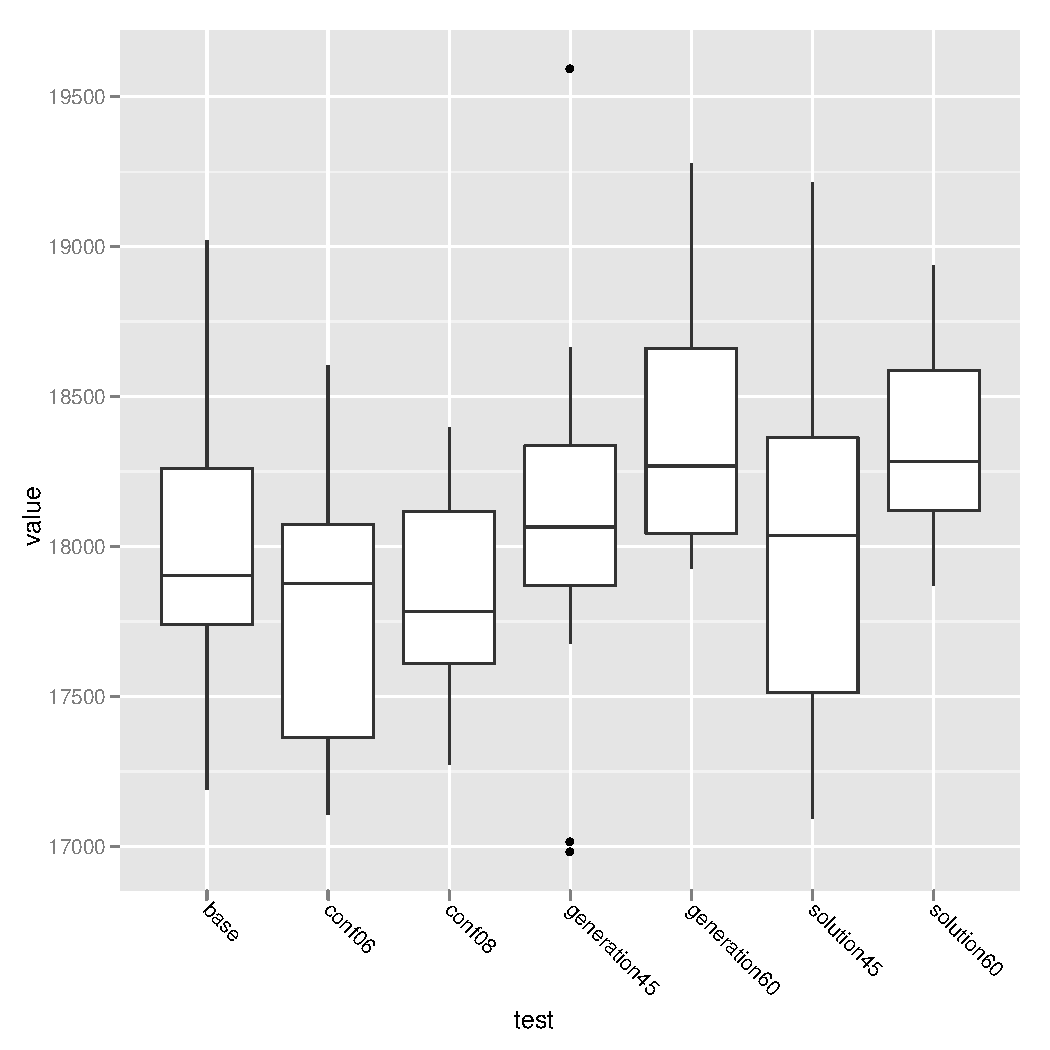
\includegraphics[width=0.6\textwidth]{exp/nouncert/c2_cont_params1b}
      \label{c2_cont_params1b}
    }
  }
  \caption{Basic parameters for the two-criteria continuous knapsack problem}
  \label{c2_cont_params}
\end{figure}

\begin{figure}
  \centering
  \makebox[\textwidth]{
    \subfloat{
      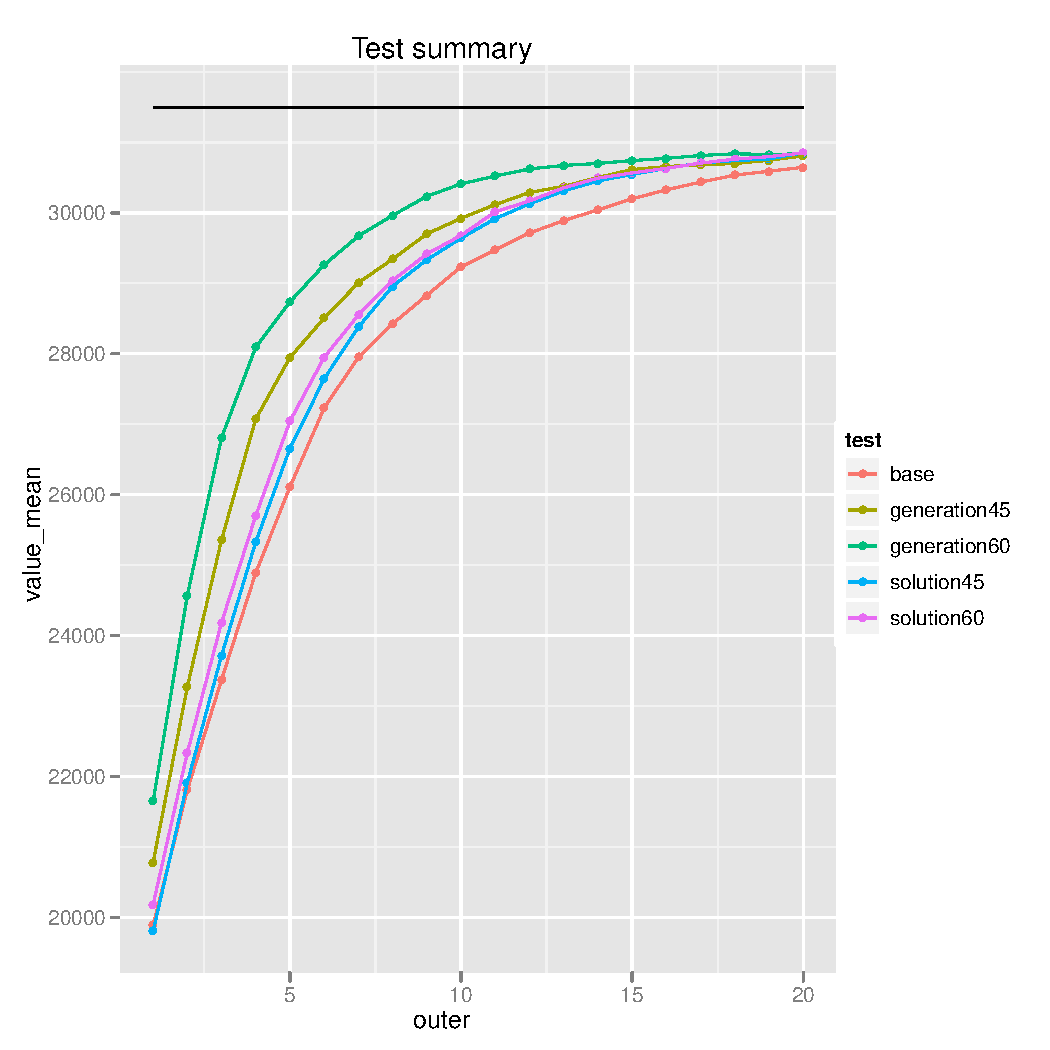
\includegraphics[width=0.65\textwidth]{exp/nouncert/c3_params1}
      \label{c3_params1}
    }
    \subfloat{
      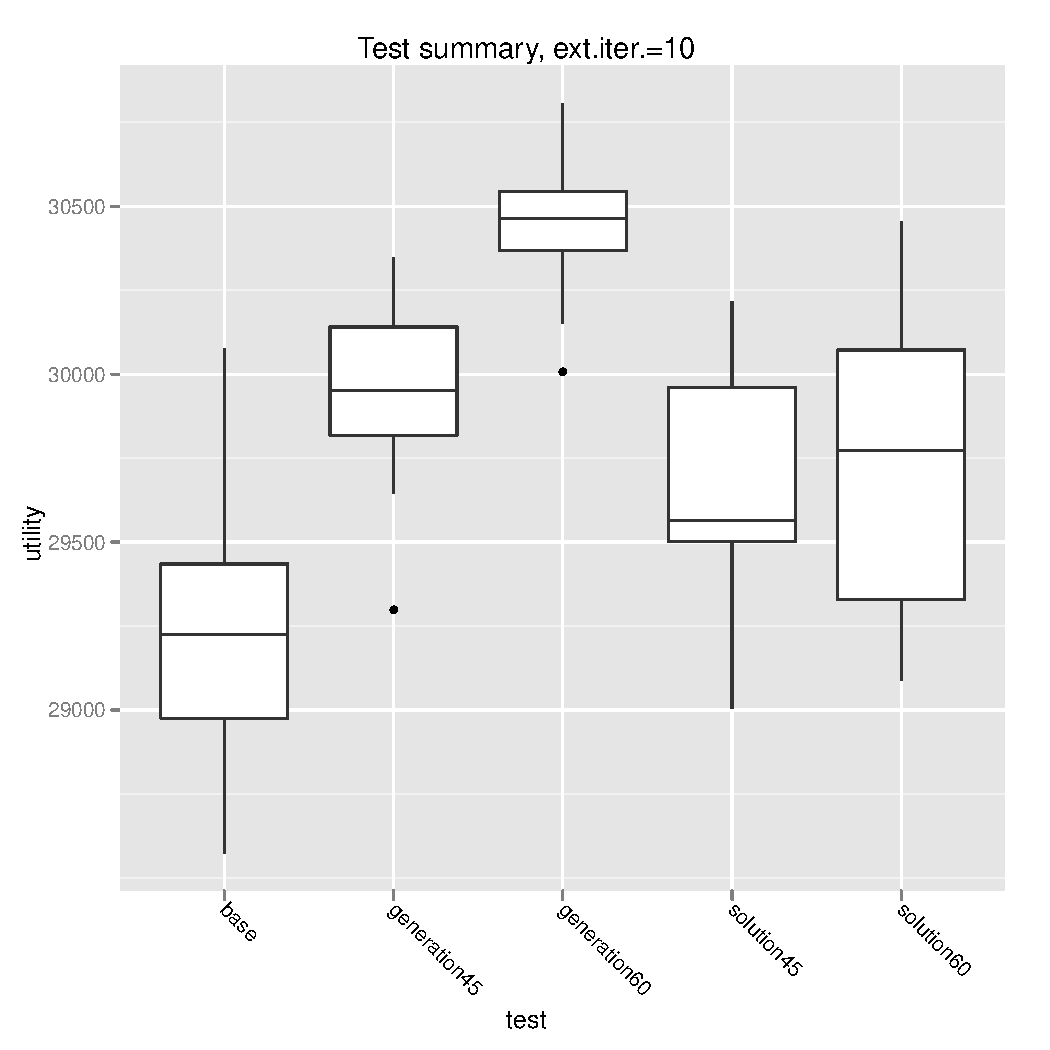
\includegraphics[width=0.6\textwidth]{exp/nouncert/c3_params1b}
      \label{c3_params1b}
    }
  }
  \caption{Basic parameters for the three-criteria binary knapsack problem}
  \label{c3_params}
\end{figure}

\begin{figure}
  \centering
  \makebox[\textwidth]{
    \subfloat{
      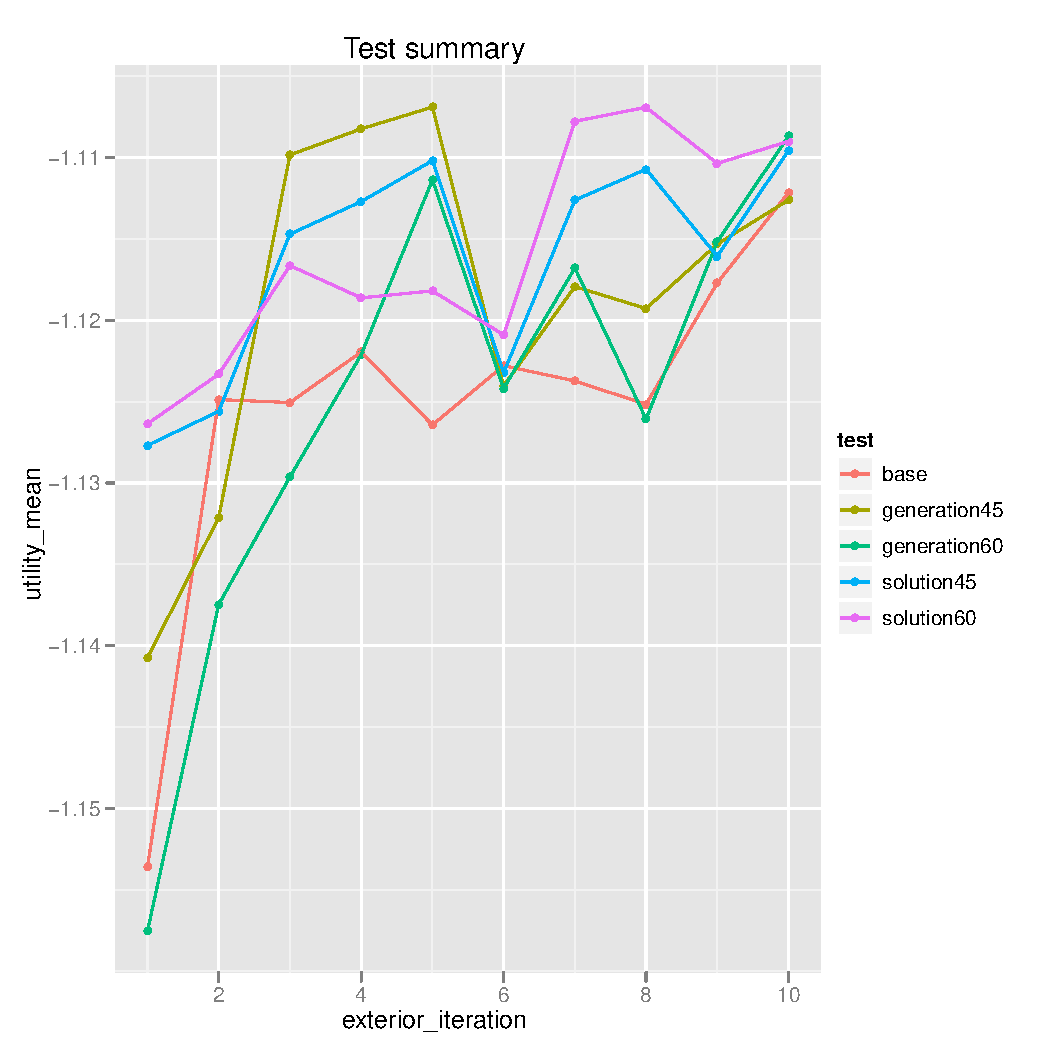
\includegraphics[width=0.65\textwidth]{exp/nouncert/c3_surface_params1}
      \label{c3_surface_params1}
    }
    \subfloat{
      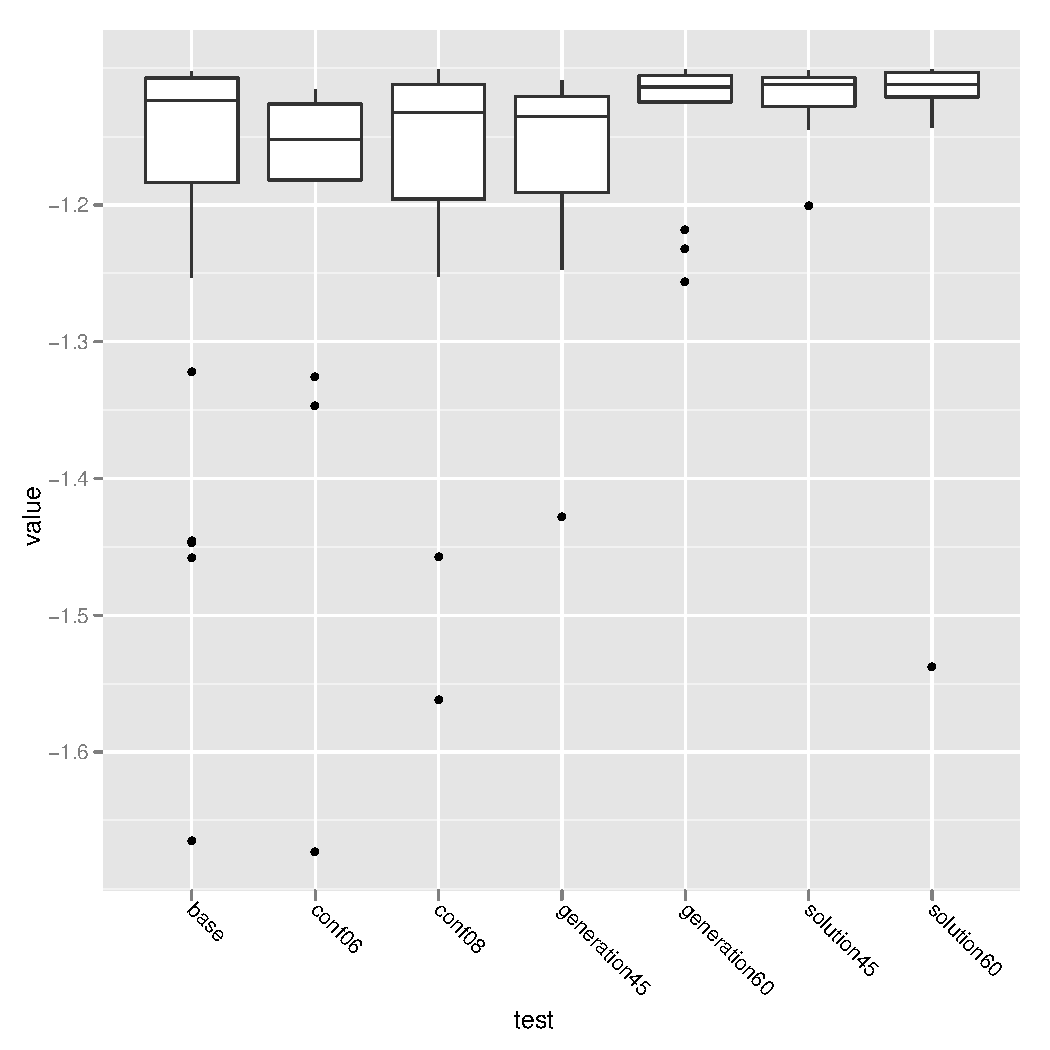
\includegraphics[width=0.6\textwidth]{exp/nouncert/c3_surface_params1b}
      \label{c3_surface_params1b}
    }
  }
  \caption{Basic parameters for the three-criteria DTLZ surface problem}
  \label{c3_surface_params}
\end{figure}


\begin{table}
  \centering
  \caption{Importance of base parameters}
  \label{t:base_imp_1}
  \begin{tabular}{r c c c c c c}
    & \multicolumn{3}{c}{Knapsack bin 2c} & \multicolumn{3}{c}{Knapsack cont 2c} \\
    \hline
    test & mean & sd & improvement & mean & sd & improvement \\
    \hline
    \hline
    base & 3870.72 & 45.73 & 0.00\% & 17968.94 & 451.61 & 0.00\% \\
    conf06 & 3865.89 & 26.77 & -0.12\% & 17781.10 & 454.59 & -1.05\% \\
    conf08 & 3855.53 & 40.73 & -0.39\% & 17831.72 & 366.52 & -0.76\% \\
    generation45 & 3958.75 & 34.14 & 2.27\% & 18072.44 & 635.22 & 0.58\% \\
    generation60 & 3995.55 & 32.71 & 3.22\% & 18366.65 & 397.56 & 2.21\% \\
    solution45 & 3937.89 & 26.11 & 1.74\% & 17950.64 & 609.37 & -0.10\% \\
    solution60 & 3924.30 & 44.31 & 1.38\% & 18341.43 & 325.21 & 2.07\% \\

    \hline
  \end{tabular}
\end{table}

\begin{table}
  \centering
  \caption{Importance of base parameters}
  \label{t:base_imp_2}
  \begin{tabular}{r c c c c c c}
    & \multicolumn{3}{c}{Knapsack bin 3c} & \multicolumn{3}{c}{DTLZ surface 3c} \\
    \hline
    test & mean & sd & improvement & mean & sd & improvement \\
    \hline
    \hline
    base & 29236.10 & 355.30 & 0.00\% & -1.19 & 0.14 & 0.00\% \\
    conf06 & 29000.25 & 431.24 & -0.81\% & -1.21 & 0.15 & 1.24\% \\
    conf08 & 28905.89 & 467.62 & -1.13\% & -1.19 & 0.14 & 0.11\% \\
    generation45 & 29923.32 & 263.40 & 2.35\% & -1.17 & 0.08 & -1.73\% \\
    generation60 & 30412.27 & 225.15 & 4.02\% & -1.14 & 0.05 & -4.61\% \\
    solution45 & 29642.44 & 362.47 & 1.39\% & -1.12 & 0.03 & -5.71\% \\
    solution60 & 29681.42 & 489.78 & 1.52\% & -1.14 & 0.11 & -4.11\% \\
    \hline
  \end{tabular}
\end{table}


Numerical data are presented in table~\ref{t:base_imp_1}
and~\ref{t:base_imp_2}. The results are also shown in charts
(fig.~\ref{c2_params}, \ref{c2_cont_params}, \ref{c3_params}
and~\ref{c3_surface_params}). This agrees with the intuition. More solutions
(individuals in the population) and longer interior loop (more generations)
will result in a better value of supposed utility for all the
problems. Confidence however yields an interesting result --- one should not
lower the confidence (the default is $100\%$).

The other parameters are:
\begin{itemize}
\item Delta ($\delta$) --- decay of a rule weight.
\item Eta ($\eta$) --- initial mutation probability.
\item Gamma ($\gamma$) --- coefficient of elitism.
\item Omega ($\omega$) --- decay rate of the mutation.
\end{itemize}

They are used in the interior loop (see~[inref]).

\begin{figure}
  \centering
  \makebox[\textwidth]{
    \subfloat[Two-criteria binary knapsack]{
      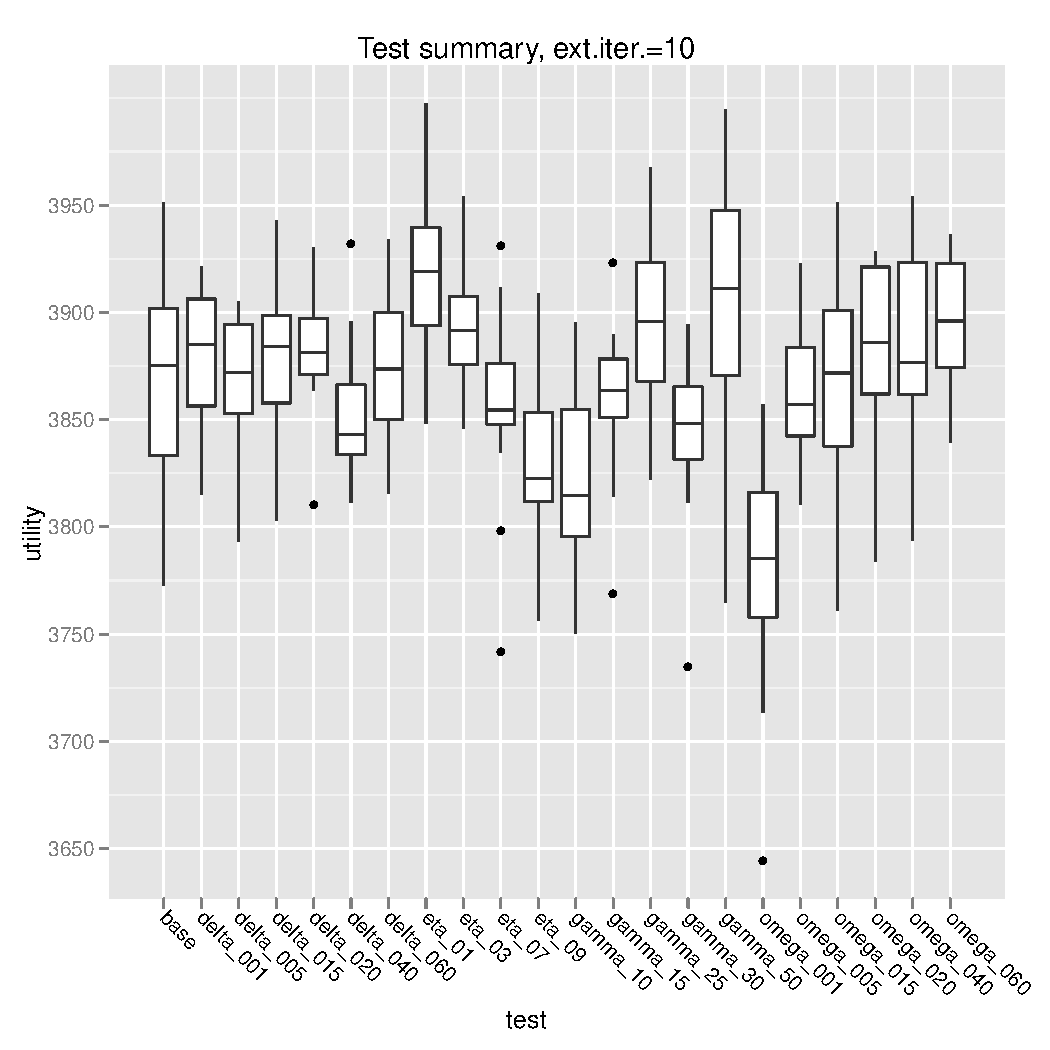
\includegraphics[width=0.60\textwidth]{exp/nouncert/c2_params2}
    }
    \subfloat[Two-criteria continuous knapsack]{
      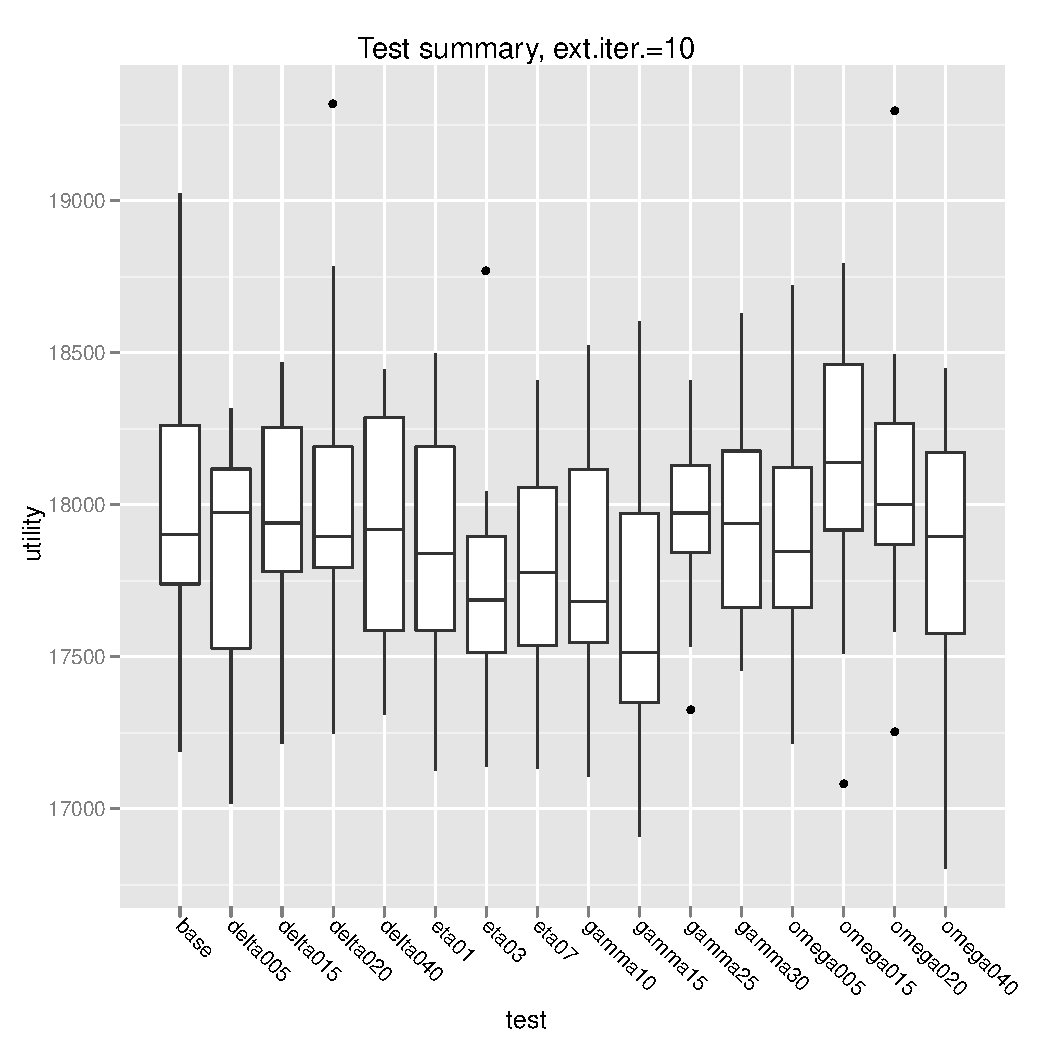
\includegraphics[width=0.60\textwidth]{exp/nouncert/c2_cont_params2}
    }
  }
  \makebox[\textwidth]{
    \subfloat[Three-criteria binary knapsack]{
      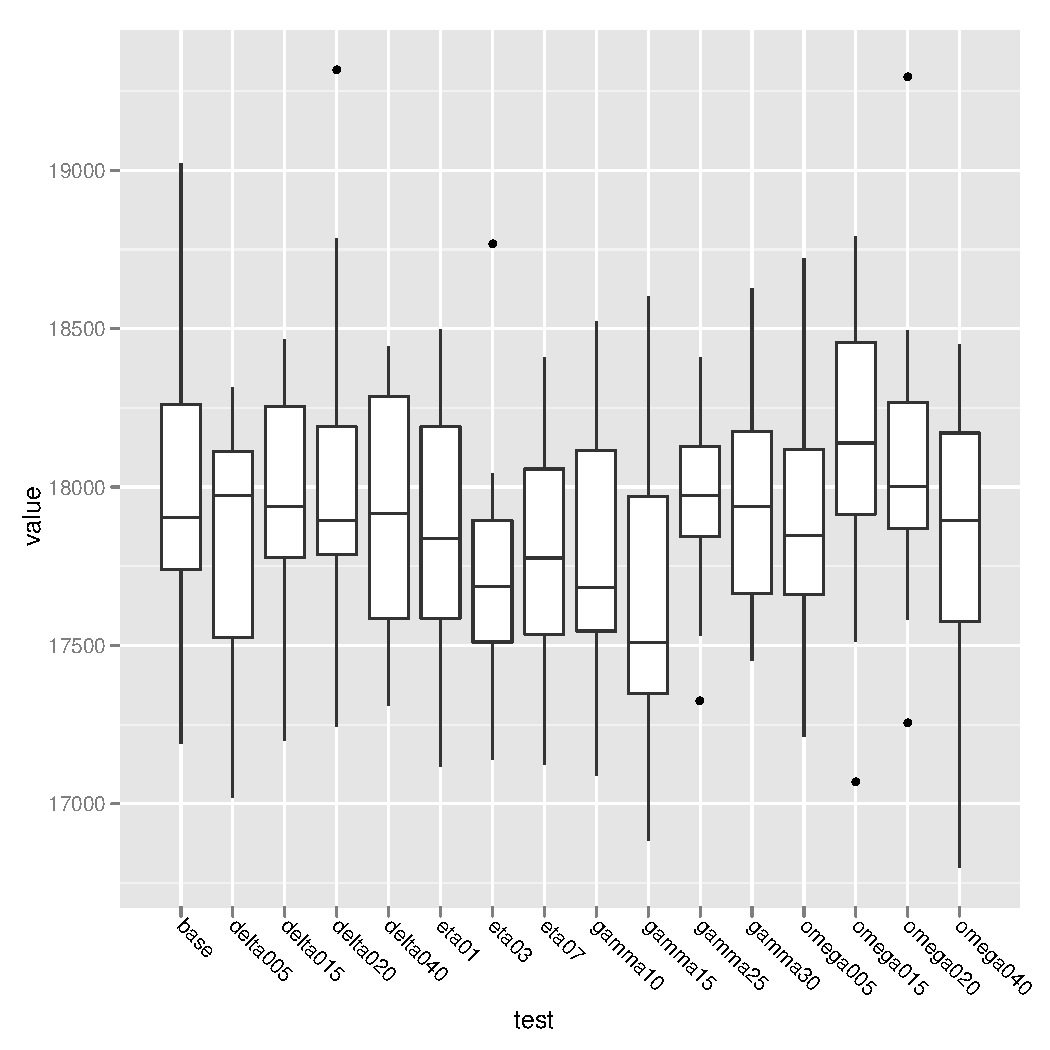
\includegraphics[width=0.60\textwidth]{exp/nouncert/c3_params2}
    }
    \subfloat[DTLZ surface problem]{
      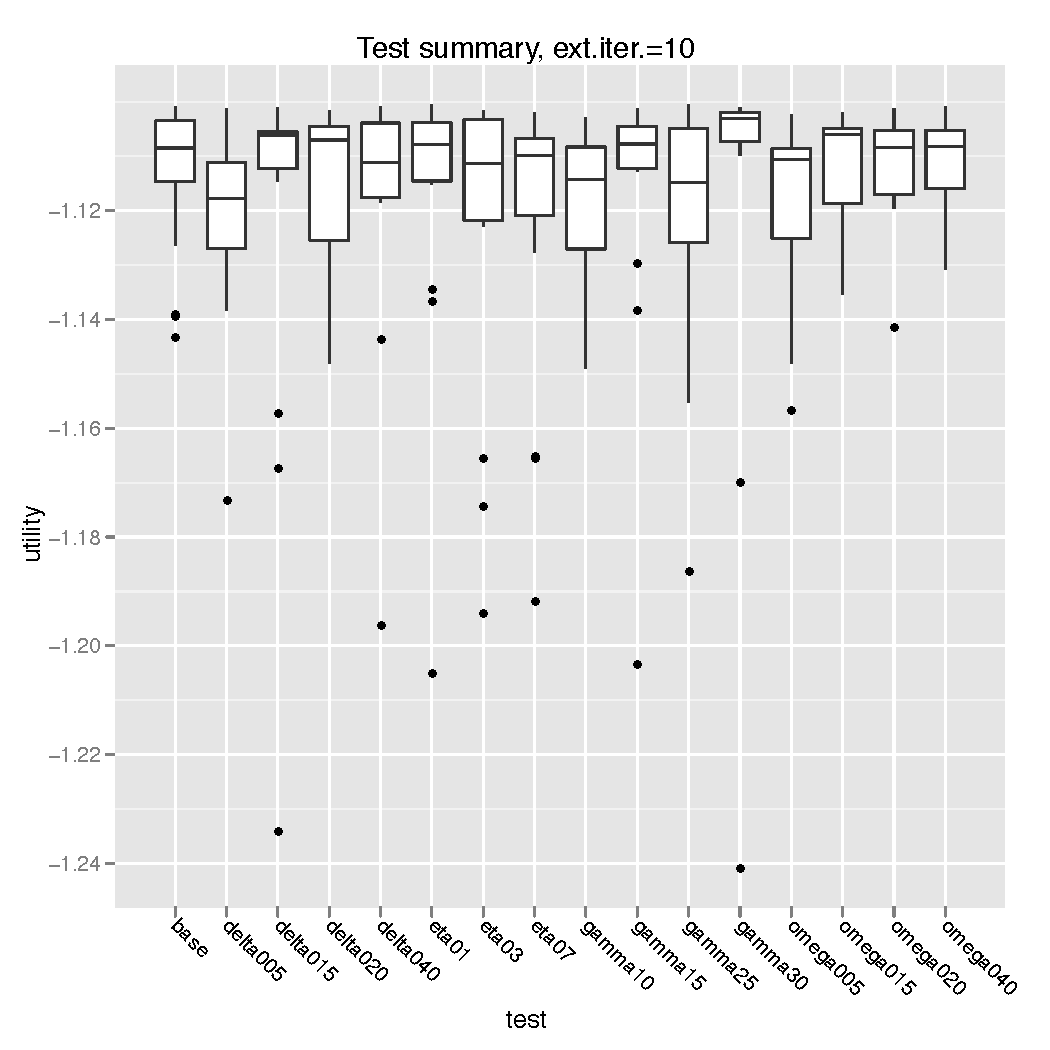
\includegraphics[width=0.60\textwidth]{exp/nouncert/c3_surface_params2}
    }
  }
  \caption{Other parameters for the three-criteria DTLZ surface problem}
  \label{params2}
\end{figure}

There is no clear pattern through the problems. In general changing the other
parameters has only a minor influence on the algorithm. This is a good thing,
because the solution given to the DM is robust with respect to those
parameters. However, analyst should try to tune the parameters on a problem
basis.

\subsection{Noise in the DM's decisions}

In the experiments performed the decision maker was mocked by a computer
algorithm. Its choices were based on the assumed supposed utility
function. They were repeatable and always complying with the assumed
function. This is not the case in a real-world situation where the DM is a
human being and the supposed utility function is not known. His or her
decisions will be noisy, not the best, sometimes even contradictory.

For this reason it is important to measure the impact of a ``noise'' in the
DM's choices on the algorithm. Normally, without introducing an artificial
noise the decisions are carried as follows:

\begin{algorithm}
\caption{Mocked DM indicating ``good'' solutions}\label{alg:dmselection}
  \begin{algorithmic}[1]
    \Procedure{SelectGoodSolutions}{solutions, toSelect} \\
    \Comment{solutions  --- a list of solutions generated in the interior
      loop} \\
    \Comment{toSelect --- how many solutions should be marked as ``good''}
    \ForAll{$s \in \text{solutions}$}
    \State $s.$value $\gets$ \Call{SupposedUtilityFunction}{$s$}
    \EndFor
    \State solutions $\gets$ \Call{Sort}{key=value, descending=True} \\
    \Comment{Sort solutions on descending supposed utility}
    \State \textbf{return} \Call{GetFirst}{solutions, toSelect}
    \EndProcedure
  \end{algorithmic}
\end{algorithm}

and the \textit{toSelect} parameter is set to $3$ so always three solutions
are marked as good. One can influence the behaviour of
\textsc{SelectGoodSolutions} by changing the toSelect parameter. But this is
not enough to simulate human-made noise.

First, note that one do not have to always select the same number of
solutions. In fact, this is unrealistic because the decision maker will select
as many solutions as he or she will think are appropriate. To mock this
behavior an additional parameter was added --- toSelectDelta. Now the number
of solutions to be selected are taken from $[\text{toSelect} -
  \text{toSelectDelta}, \text{toSelect} + \text{toSelectDelta}]$ with uniform
distribution.

Furthermore, the human decision maker is fallible. He or she can make a wrong
decision and not select the best solutions according to the supposed utility
function. Another parameter was introduced to simulate this phenomenon ---
noiseLimit. After sorting the solutions on the basis of the supposed utility
value the individuals $1, 2, \dots, \text{noiseLimit}$ are shuffled. Supposing
one wants to select three solutions. If the noiseLimit parameter is set to $0$
(the default) three best solutions will be selected. However, if an
experimenter sets the noiseLimit to $6$, then $3$ out of $6$ best solutions
will be picked by random.

The noisy version of the algorithm~\ref{alg:dmselection} is shown below.
\begin{algorithm}
\caption{Mocked DM indicating ``good'' solutions}\label{alg:noisydmselection}
  \begin{algorithmic}[1]
    \Procedure{NoisySelectGoodSolutions}{solutions, toSelect, toSelectDelta, 
      noiseLimit}
    \ForAll{$s \in \text{solutions}$}
    \State $s.$value $\gets$ \Call{SupposedUtilityFunction}{$s$}
    \EndFor
    \State solutions $\gets$ \Call{Sort}{key=value, descending=True}
    \State shuffled $\gets$ \Call{ShuffleFirst}{solutions, noiseLimit}
    \State toSelect$' \gets$ \Call{RandomFromInterval}{toSelect $-$
      toSelectDelta, toSelect $+$ toSelectDelta}
    \State \textbf{return} \Call{GetFirst}{shuffled, toSelect$'$}
    \EndProcedure
  \end{algorithmic}
\end{algorithm}

Following tests were performed:

\begin{tabular}{r c c c c c c c}
  \hline
  Parameter & no noise & noise$_1$ & noise$_2$ & noise$_3$ & noise$_4$ &
  noise$_5$ & noise$_6$ \\
  \hline
  \hline
  toSelect      & 3 & 3 & 3 & 3 & 5 &  3 &  3 \\
  toSelectDelta & 0 & 2 & 2 & 2 & 4 &  4 &  2 \\
  noiseLimit    & 0 & 0 & 2 & 4 & 6 & 10 & 16 \\
  \hline \\
\end{tabular}

Note that noise$_1$ to noise$_4$ are rather minor ones, noise$_5$ is medium
noise and finally noise$_6$ is a big one, unlikely to happen in practice ---
half of the solutions are considered good. If the decision maker is careful in
his or her evaluations, the algorithm will probably have to face a noise
between $1$ and $4$.

The results for the exemplary problems are shown in the charts below
(fig.~\ref{c2_noise}, \ref{c3_noise} and \ref{c3_surface_noise}). Noise tests
for the continuous knapsack are omitted --- the algorithm performs badly even
without additional noise.

\begin{figure}
  \centering
  \makebox[\textwidth]{
    \subfloat{
      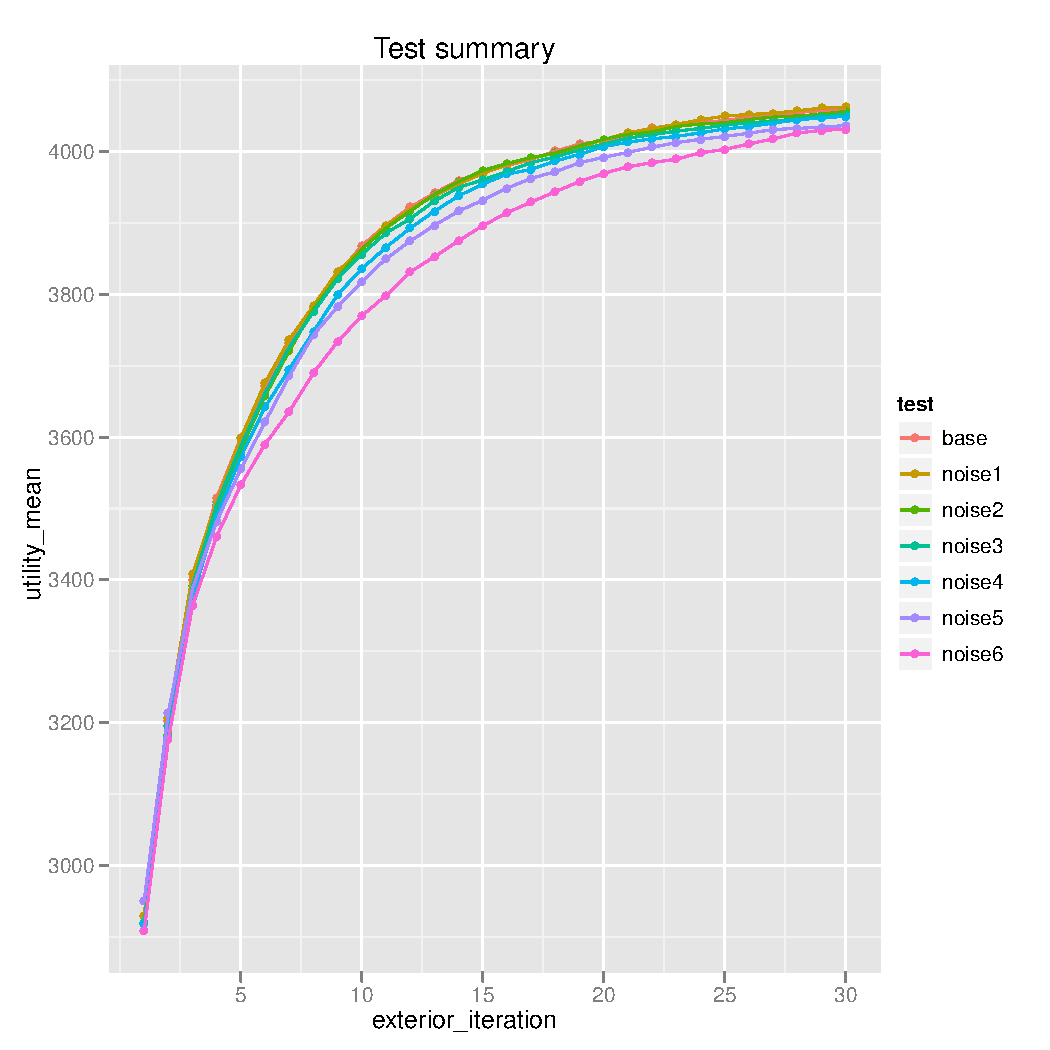
\includegraphics[width=0.65\textwidth]{exp/nouncert/c2_noise}
      \label{c2_noisea}
    }
    \subfloat{
      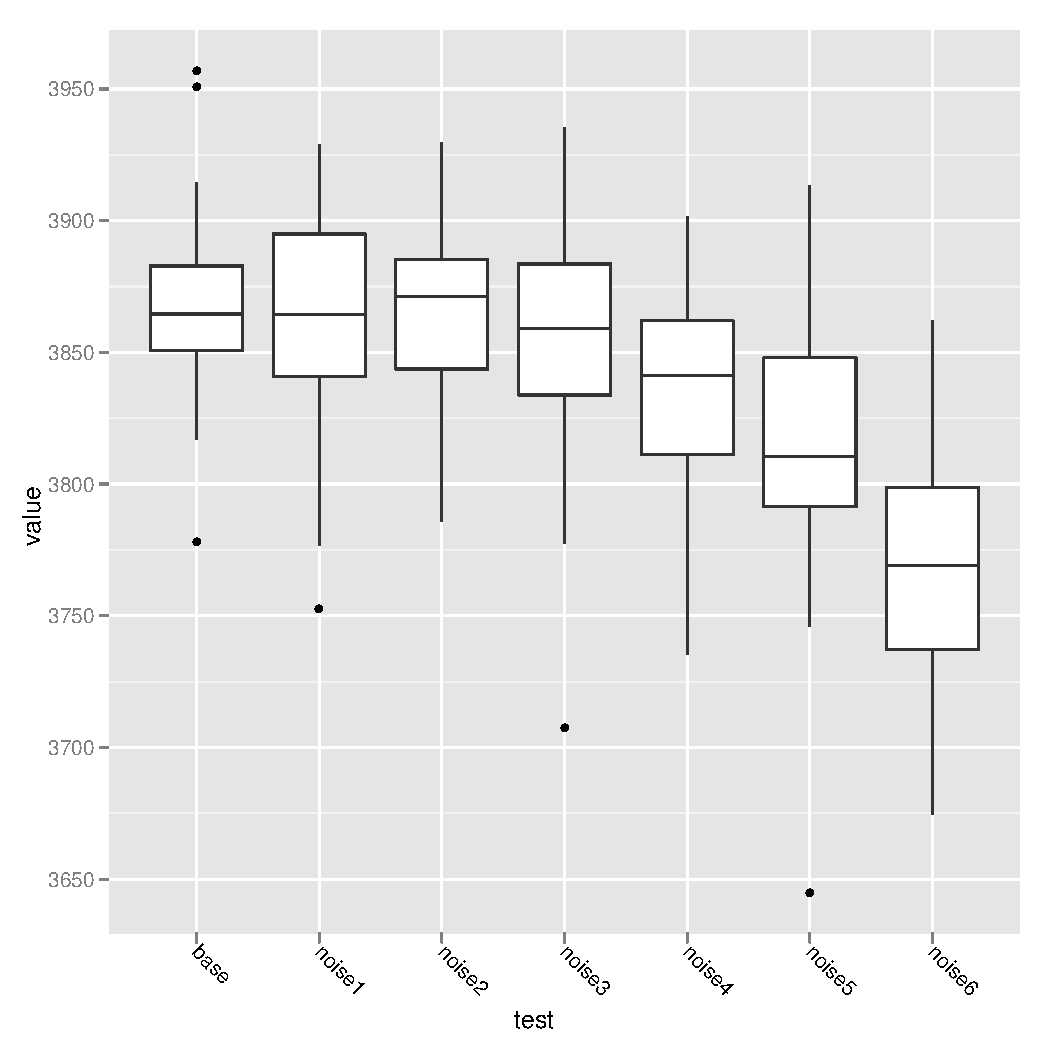
\includegraphics[width=0.65\textwidth]{exp/nouncert/c2_noiseb}
      \label{c2_noiseb}
    }
  }
  \caption{The impact of noise for the two-criteria binary knapsack problem}
  \label{c2_noise}
\end{figure}

\begin{figure}
  \centering
  \makebox[\textwidth]{
    \subfloat{
      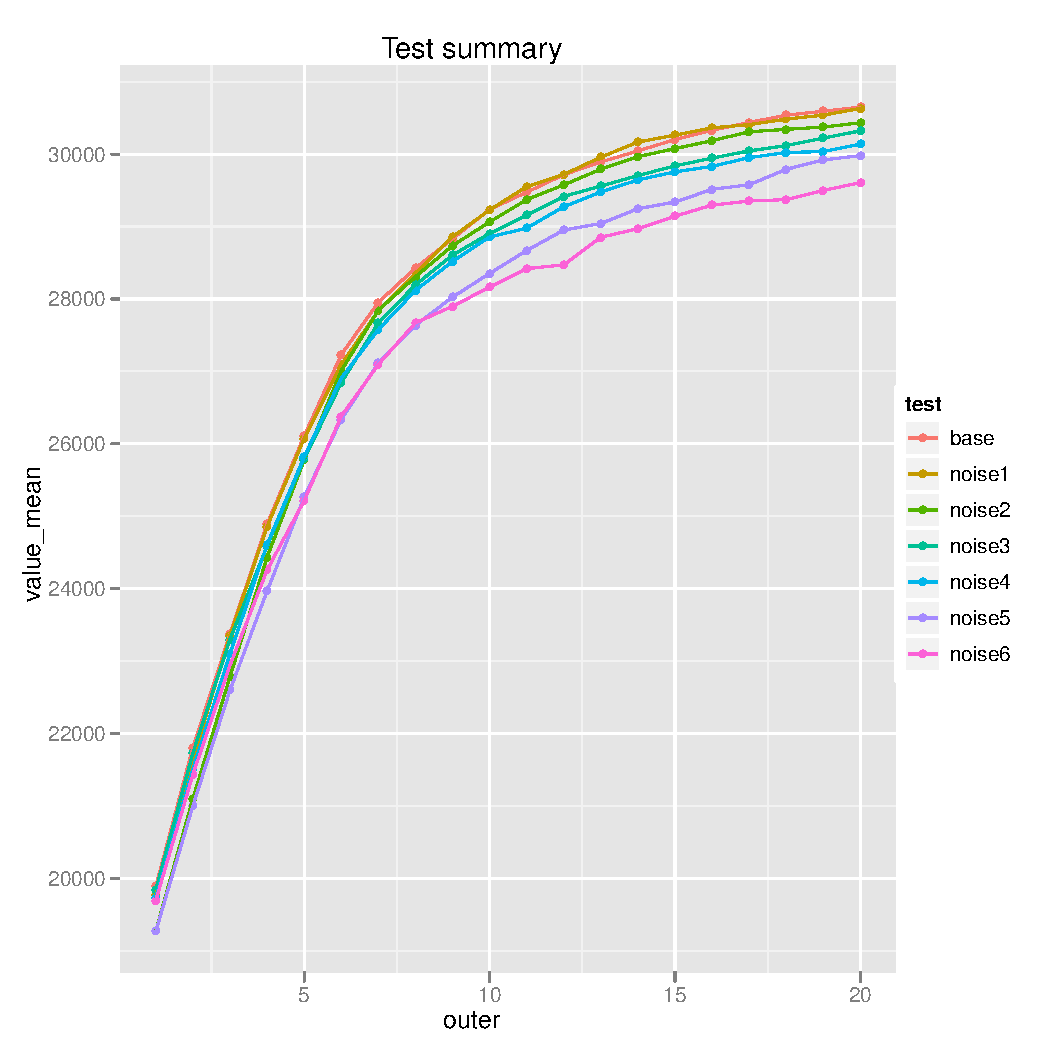
\includegraphics[width=0.65\textwidth]{exp/nouncert/c3_noise}
      \label{c3_noisea}
    }
    \subfloat{
      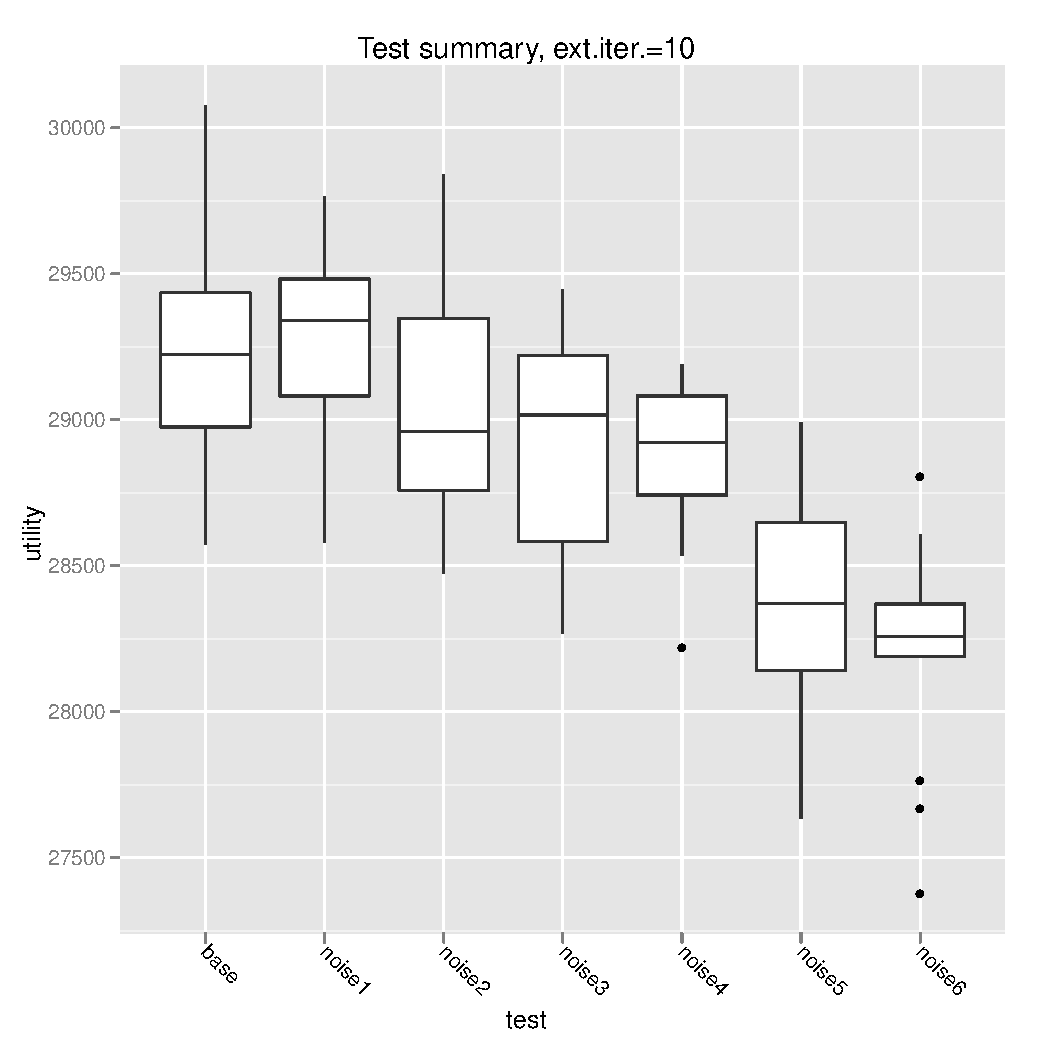
\includegraphics[width=0.65\textwidth]{exp/nouncert/c3_noiseb}
      \label{c3_noiseb}
    }
  }
  \caption{The impact of noise for the three-criteria binary knapsack problem}
  \label{c3_noise}
\end{figure}

\begin{figure}
  \centering
  \makebox[\textwidth]{
    \subfloat{
      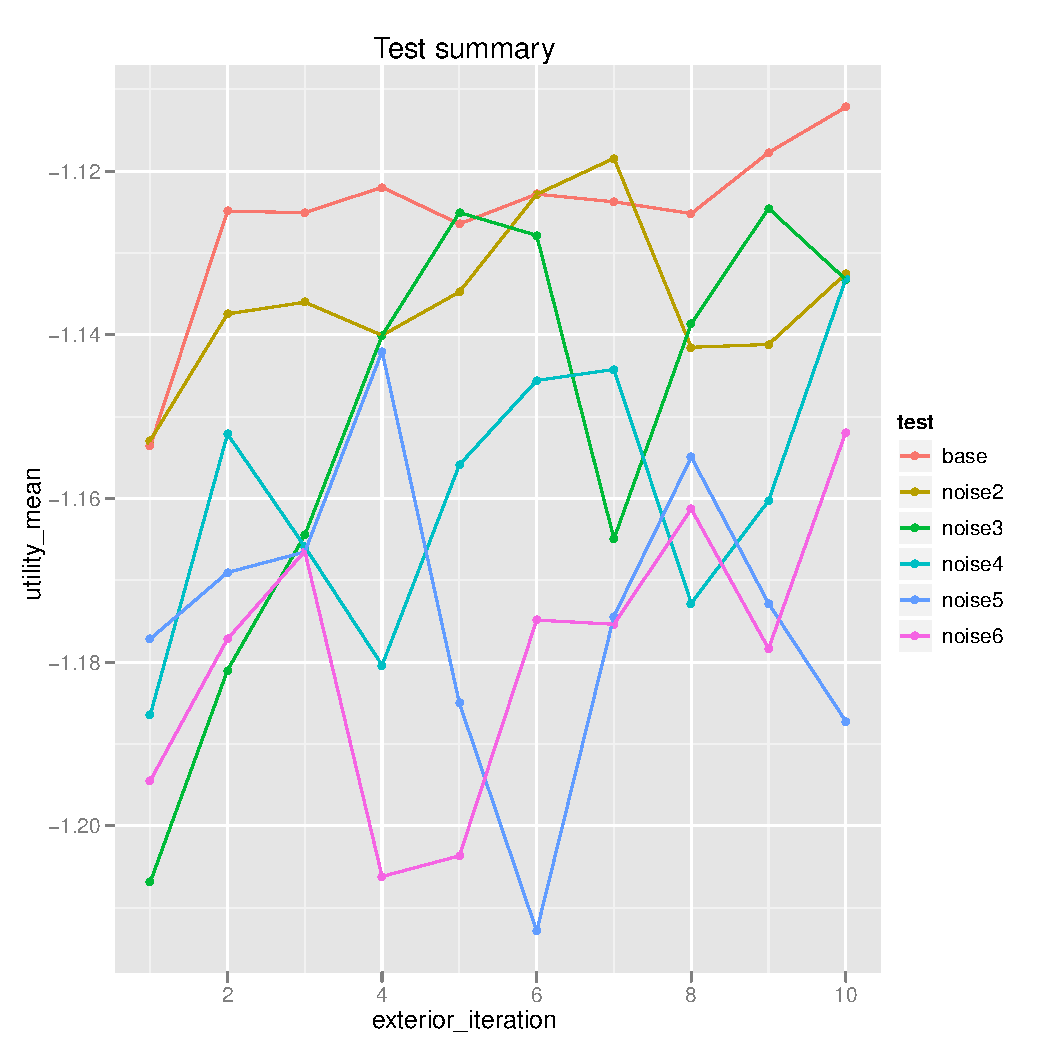
\includegraphics[width=0.65\textwidth]{exp/nouncert/c3_surface_noise}
      \label{c3_surface_noisea}
    }
    \subfloat{
      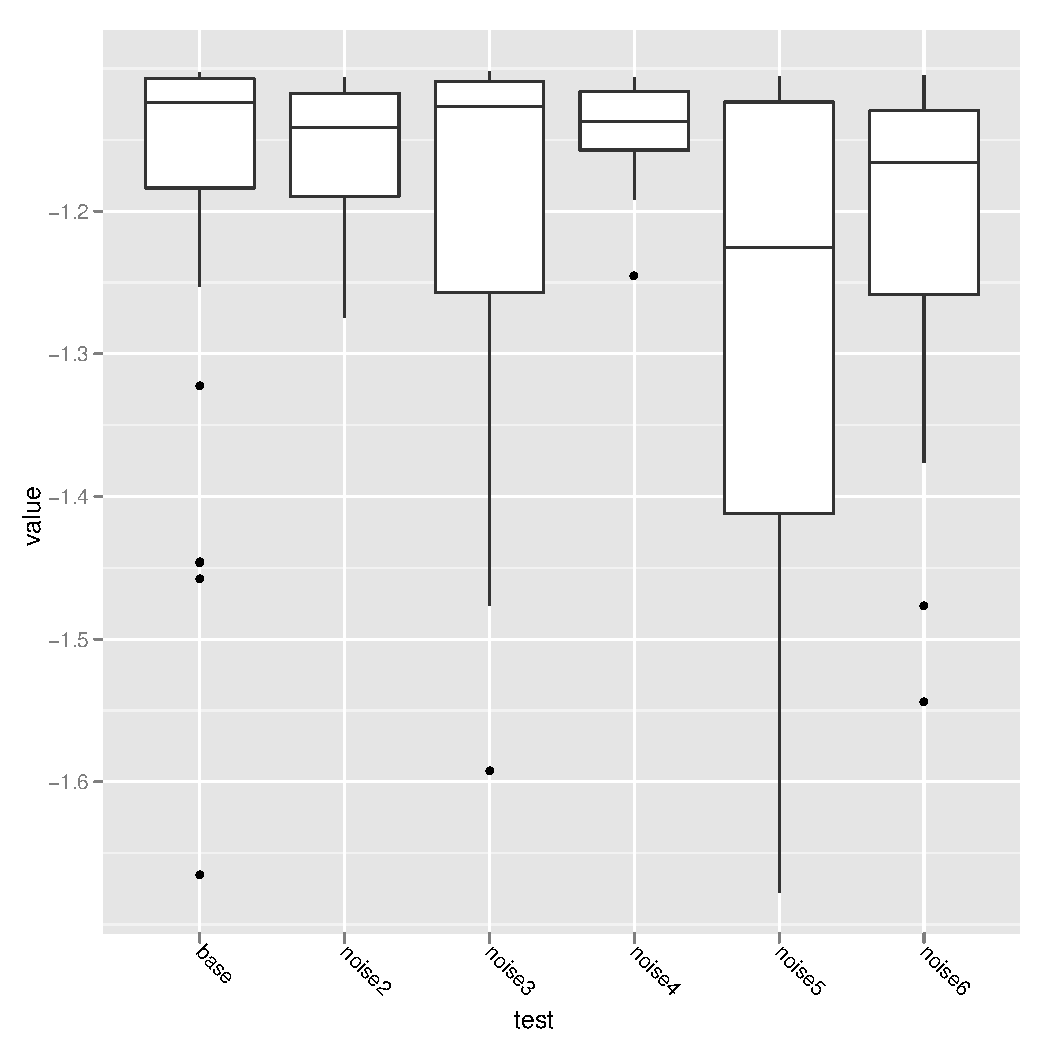
\includegraphics[width=0.65\textwidth]{exp/nouncert/c3_surface_noiseb}
      \label{c3_surface_noiseb}
    }
  }
  \caption{The impact of noise for the three-criteria DTLZ surface problem}
  \label{c3_surface_noise}
\end{figure}

Results of the DTLZ surface problem (table~\ref{t:noise1}, \ref{t:noise2} and
fig.\ref{c3_surface_noise}) are inconclusive. This is because of the behavior
described in section~\ref{nouncert-performance} --- the decision rules are not
discriminating enough so that often the utility value drops between the
interior loops. This can be seen as a form of noise with even bigger impact
than the one tested here, so it obscures results for this particular problem.

For the other problems however --- binary knapsacks (fig.~\ref{c2_noise} and
\ref{c3_noise}) the results are clear. Minor noises make almost no harm to the
results, while medium and major have only a small impact --- the value has
decreased less than $5\%$ after ten iterations. This means that the solution
generated by the DARWIN is robust with respect to the noise in the decision
maker's choices. Even with the major noise the algorithm is able to provide the
same results, however a few iterations later.

\begin{table}[h]
  \centering
  \caption{The impact of noise on knapsack bin 2c}
  \label{t:noise1}
  \begin{tabular}{r c c c}
    \hline
    noise level & mean & sd & improvement\\
    \hline
    \hline
    base & 3867.66 & 37.12 & 0.00\% \\
    noise1 & 3863.02 & 42.34 & -0.12\% \\
    noise2 & 3862.67 & 35.92 & -0.13\% \\
    noise3 & 3854.10 & 46.61 & -0.35\% \\
    noise4 & 3833.94 & 44.61 & -0.87\% \\
    noise5 & 3814.34 & 50.59 & -1.38\% \\
    noise6 & 3767.85 & 46.63 & -2.58\% \\
    \hline
  \end{tabular}
\end{table}

\begin{table}[h]
  \centering
  \caption{The impact of noise on knapsack bin 3c}
  \label{t:noise2}
  \begin{tabular}{r c c c}
    \hline
    noise level & mean & sd & improvement\\
    \hline
    \hline
    base & 29236.10 & 355.30 & 0.00\% \\
    noise1 & 29228.82 & 339.02 & -0.02\% \\
    noise2 & 29063.68 & 422.31 & -0.59\% \\
    noise3 & 28903.57 & 388.95 & -1.14\% \\
    noise4 & 28855.74 & 253.07 & -1.30\% \\
    noise5 & 28352.64 & 398.55 & -3.02\% \\
    noise6 & 28163.63 & 383.71 & -3.67\% \\
    \hline
  \end{tabular}
\end{table}

\begin{table}[h]
  \centering
  \caption{The impact of noise on DTLZ surface 3c}
  \label{t:noise3}
  \begin{tabular}{r c c c}
    \hline
    test & mean & sd & improvement  \\
    \hline
    \hline
    base & -1.19 & 0.14 & 0.00\%     \\
    noise2 & -1.16 & 0.05 & 2.65\%   \\
    noise3 & -1.21 & 0.15 & -1.46\%  \\
    noise4 & -1.14 & 0.04 & 3.88\%   \\
    noise5 & -1.28 & 0.17 & -7.66\%  \\
    noise6 & -1.21 & 0.11 & -1.75\%  \\
    \hline
  \end{tabular}
\end{table}

\clearpage{}
